\section{Free entry and the number of firms}\label{sec:02-entry}

\Cref{sec:02-cournot} took the number of firms as given. In most industries the number of firms is itself an
equilibrium outcome. Firms enter while the profit of one more entrant covers the cost of setting up, and they stay
out once it does not. This section asks whether free entry delivers the number of firms that maximizes total surplus.
The general answer, due to \citet{MankiwWhinston1986}, is that in homogeneous-good markets with imperfect competition
free entry tends to produce too many firms. The reason is a \emph{business-stealing externality}: an entrant takes
sales from incumbents and counts them as its own profit, while society gains nothing from the transfer.

\subsection{The two-stage entry game}\label{sec:02-entry-game}

\begin{definition}[Two-stage entry game]\label{def:02-entry-game}
A large pool of identical potential entrants plays two stages. In stage~1 each potential entrant decides whether to
enter. Entry requires a \emph{set-up cost} $F > 0$, which is sunk once paid. In stage~2 the $N$ entrants observe
$N$ and play an oligopoly game in output or prices. Each entrant has the cost function $C(q)$, with $C$ continuous,
$C(0) = 0$, $C' \ge 0$ and $C'' \ge 0$. The stage-2 game has a symmetric equilibrium in which each firm produces
$q_N$ and the price is $P(N q_N)$. The \emph{per-firm profit} with $N$ entrants, net of the set-up cost, is
\begin{equation}\label{eq:02-entry-profit}
\pi_N = P(N q_N)\, q_N - C(q_N) - F .
\end{equation}
The solution concept is subgame-perfect equilibrium (\cref{def:02-spe}).
\end{definition}

The definition leaves the stage-2 game open. It may be Cournot, Bertrand, a cartel, or any other game with a
symmetric outcome. This generality is the main strength of the analysis that follows.

The \emph{free-entry number of firms} $N^e$ satisfies two conditions \citep[p.~50]{MankiwWhinston1986}:
\begin{equation}\label{eq:02-free-entry}
\pi_{N^e} \ge 0 \qquad\text{and}\qquad \pi_{N^e + 1} < 0 .
\end{equation}
The first condition says that no entrant regrets entering. The second says that no outsider wishes to enter. A firm
that is indifferent enters. When we treat $N$ as a continuous variable, the two conditions collapse to the
zero-profit condition $\pi_{N^e} = 0$.

\begin{example}[Free entry in the linear Cournot market]\label{ex:02-free-entry-linear}
Let $P(Q) = a - bQ$ and $C(q) = cq$, with $a > c \ge 0$ and $b > 0$, and let the entrants play Cournot.
\Cref{ex:02-linear-cournot} gives
\begin{equation*}
q_N = \frac{a - c}{b(N + 1)}, \qquad P - c = \frac{a - c}{N + 1} = b\, q_N, \qquad
\pi_N = \frac{(a - c)^2}{b(N + 1)^2} - F .
\end{equation*}
Setting $\pi_{N^e} = 0$ and solving for $N^e$ gives
\begin{equation}\label{eq:02-Ne-linear}
(N^e + 1)^2 = \frac{(a - c)^2}{bF}
\qquad\Longrightarrow\qquad
N^e = \frac{a - c}{\sqrt{bF}} - 1 .
\end{equation}
At least one firm enters when $F \le \frac{(a - c)^2}{4b}$. Substituting $\frac{a - c}{N^e + 1} = \sqrt{bF}$ into
the Cournot formulas gives the free-entry outcome:
\begin{gather*}
P^e = c + \sqrt{bF}, \qquad q^e = \sqrt{\frac{F}{b}}, \qquad Q^e = \frac{a - c - \sqrt{bF}}{b}, \\
L^e = \frac{\sqrt{bF}}{c + \sqrt{bF}}, \qquad \HHI^e = \frac{1}{N^e} = \frac{\sqrt{bF}}{a - c - \sqrt{bF}} .
\end{gather*}
They fill the free-entry column of \cref{tab:02-linear-cournot}. As a check, $(P^e - c)\, q^e = \sqrt{bF}
\sqrt{\frac{F}{b}} = F$, so operating profit just covers the set-up cost.
\end{example}

The example makes two points. First, under free entry the price-cost margin equals $\sqrt{bF}$ exactly. Markups are
what pays for fixed costs, which is the point of \cref{rem:02-fixed-costs}. A positive
Lerner index is therefore compatible with zero economic profit. Second, the margin does not depend on the demand
intercept $a$. A higher intercept attracts more firms and leaves the margin unchanged, while concentration falls.
Adding consumers is different. Scaling the number of consumers by $M$ replaces $b$ by $\frac{b}{M}$, so the
free-entry margin $\sqrt{\frac{bF}{M}}$ falls as the market grows (\cref{tab:02-LH-cases}).

\subsection{The second-best planner and excess entry}\label{sec:02-mw}

\citet{MankiwWhinston1986} compare $N^e$ with the choice of a \emph{second-best planner}. This planner chooses how
many firms enter but cannot control how they compete after entry. The restriction reflects antitrust practice.
\citet[p.~50]{MankiwWhinston1986} quote the observation of \citet[p.~525]{Scherer1980} that oligopolists who
refrain from price competition, each deciding independently, do not break the law. The planner maximizes total
surplus, ignoring income effects:
\begin{equation}\label{eq:02-mw-welfare}
W(N) = \int_0^{N q_N} P(x)\, \dd x - N\, C(q_N) - N F .
\end{equation}
The first term is gross consumer benefit, and the last two are production and set-up costs. Prices are transfers
between consumers and firms, so they do not appear. Let $N^o$ denote the maximizer of $W$ (Mankiw and Whinston
write $N^*$). With continuous $N$ it satisfies $W'(N^o) = 0$.

\begin{assumption}[Post-entry outcomes]\label{ass:02-mw}
The symmetric stage-2 outcomes satisfy the following conditions \citep[p.~51]{MankiwWhinston1986}.
\begin{enumerate}[label=(E\arabic*)]
\item Total output rises with $N$ and stays bounded: $N q_N > N' q_{N'}$ for all $N > N'$, and
  $\lim_{N\to\infty} N q_N = Q_\infty < \infty$.
\item Per-firm output falls with $N$: $q_N < q_{N'}$ for all $N > N'$.
\item Price is not below marginal cost: $P(N q_N) - C'(q_N) \ge 0$ for all $N$.
\end{enumerate}
When $N$ is continuous we also assume that $q_N$ is differentiable, with $\frac{\dd q_N}{\dd N} < 0 <
\frac{\dd (N q_N)}{\dd N}$.
\end{assumption}

Condition (E2) is the \emph{business-stealing effect}: an entrant lowers the equilibrium output of each incumbent.
\Cref{prop:02-entry-cs} and the derivatives \eqref{eq:02-seade} show that Cournot competition satisfies (E1) and
(E2) under \cref{ass:02-cournot}. Condition
(E3) holds for any conduct between price taking and monopoly. Business stealing is closely related to quantities
being strategic substitutes \citep{BulowGeanakoplosKlemperer1985}, and \citet{Seade1980} gives conditions for it
under conjectural variations.

\begin{proposition}[Excess entry]\label{prop:02-mw-excess}
Suppose \cref{ass:02-mw} holds and treat $N$ as continuous, so that $\pi_{N^e} = 0$ and $W'(N^o) = 0$. Then
$N^e \ge N^o$. If in addition $P(N^o q_{N^o}) - C'(q_{N^o}) > 0$, then $N^e > N^o$
\citep[Proposition~1]{MankiwWhinston1986}.
\end{proposition}

\begin{proof}
The proof has four steps.

\emph{Step 1.} We differentiate welfare. By the fundamental theorem of calculus and the chain rule,
\begin{equation*}
\frac{\dd}{\dd N}\int_0^{N q_N} P(x)\,\dd x = P(N q_N)\,\frac{\dd (N q_N)}{\dd N}
= P(N q_N)\left[q_N + N \frac{\dd q_N}{\dd N}\right].
\end{equation*}
The product rule gives $\frac{\dd}{\dd N}\left[N C(q_N)\right] = C(q_N) + N C'(q_N)\frac{\dd q_N}{\dd N}$. Hence
\begin{equation}\label{eq:02-mw-wprime-raw}
W'(N) = P(N q_N)\left[q_N + N\frac{\dd q_N}{\dd N}\right] - C(q_N) - N C'(q_N)\frac{\dd q_N}{\dd N} - F .
\end{equation}

\emph{Step 2.} We regroup. The terms $P(N q_N)q_N - C(q_N) - F$ add up to $\pi_N$. The remaining terms share the factor
$N\frac{\dd q_N}{\dd N}$. Therefore
\begin{equation}\label{eq:02-mw-wprime}
W'(N) = \pi_N + N\left[P(N q_N) - C'(q_N)\right]\frac{\dd q_N}{\dd N} .
\end{equation}

\emph{Step 3.} We sign the wedge. By (E3) the bracket is nonnegative. By (E2) the derivative $\frac{\dd q_N}{\dd N}$ is
negative. The second term of \eqref{eq:02-mw-wprime} is therefore nonpositive, and $W'(N) \le \pi_N$ for every $N$.
At $N = N^o$ this gives $0 = W'(N^o) \le \pi_{N^o}$. The inequality is strict when the bracket is positive at $N^o$.

\emph{Step 4.} Profit falls with entry. Differentiating \eqref{eq:02-entry-profit} gives
\begin{equation}\label{eq:02-mw-dpi}
\frac{\dd \pi_N}{\dd N} = \left[P(N q_N) - C'(q_N)\right]\frac{\dd q_N}{\dd N}
+ q_N P'(N q_N)\,\frac{\dd (N q_N)}{\dd N} .
\end{equation}
The first term is nonpositive by (E2) and (E3). The second is negative because $P' < 0$ and total output rises with
$N$. So $\pi_N$ is strictly decreasing. Since $\pi_{N^o} \ge 0 = \pi_{N^e}$, we conclude that $N^e \ge N^o$. If
$\pi_{N^o} > 0$, then $N^e > N^o$.
\end{proof}

Equation \eqref{eq:02-mw-wprime} contains the whole economics of the result. The social value of a marginal entrant
has two parts. The first is the entrant's own profit $\pi_N$, which is also its private value of entry. The second is
the surplus lost on the output that incumbents give up. Entry shrinks incumbents' total output by
$N\left|\frac{\dd q_N}{\dd N}\right|$. Each lost unit was worth $P$ to consumers and cost $C'$ to make, so each one
destroys $P - C'$ of surplus. The entrant ignores this loss. The lower price that consumers pay on the remaining units
is a transfer from incumbents, so it cancels in total surplus. \Cref{fig:02-entry} plots the two values for the
linear Cournot market.

\begin{corollary}[Price-taking entrants]\label{cor:02-mw-pricetaking}
Suppose (E1) and (E2) hold and $P(N q_N) = C'(q_N)$ for all $N$. Treating $N$ as continuous, free entry yields the
optimal number of firms, $N^e = N^o$ \citep[Corollary~1]{MankiwWhinston1986}.
\end{corollary}

\begin{proof}
With $P = C'$ the second term of \eqref{eq:02-mw-wprime} vanishes, so $W'(N) = \pi_N$ for all $N$. Hence $W'(N^o) = 0$
if and only if $\pi_{N^o} = 0$, and $N^o = N^e$.
\end{proof}

Business stealing still occurs under price taking, but the stolen units carry no surplus at the margin, since price
equals marginal cost. In this case the second-best optimum is also the first-best optimum
\citep[n.~6]{MankiwWhinston1986}. If (E2) were reversed, so that entry raised incumbents' output, the wedge in
\eqref{eq:02-mw-wprime} would be positive and free entry would produce too few firms \citep[n.~7]{MankiwWhinston1986}.

\begin{example}[Excess entry in the linear Cournot market]\label{ex:02-mw-linear}
Return to \cref{ex:02-free-entry-linear}, which is Example~1 of \citet{MankiwWhinston1986}. The free-entry number of
firms satisfies \eqref{eq:02-Ne-linear}. To find $N^o$, compute the wedge in \eqref{eq:02-mw-wprime}:
\begin{equation*}
P - c = \frac{a - c}{N + 1}, \qquad \frac{\dd q_N}{\dd N} = -\frac{a - c}{b(N + 1)^2}, \qquad
N\left[P - c\right]\frac{\dd q_N}{\dd N} = -\frac{N(a - c)^2}{b(N + 1)^3} .
\end{equation*}
Adding $\pi_N$ and collecting terms over the common denominator $b(N + 1)^3$:
\begin{align*}
W'(N) &= \frac{(a - c)^2}{b(N + 1)^2} - F - \frac{N(a - c)^2}{b(N + 1)^3} \\
&= \frac{(a - c)^2\left[(N + 1) - N\right]}{b(N + 1)^3} - F \\
&= \frac{(a - c)^2}{b(N + 1)^3} - F .
\end{align*}
$W'$ is decreasing in $N$, so $W$ is concave and its maximizer solves $W'(N^o) = 0$:
\begin{equation}\label{eq:02-No-linear}
(N^o + 1)^3 = \frac{(a - c)^2}{bF} .
\end{equation}
Comparing \eqref{eq:02-Ne-linear} with \eqref{eq:02-No-linear} gives
\begin{equation}\label{eq:02-Ne-No}
N^e + 1 = (N^o + 1)^{\frac{3}{2}} .
\end{equation}
If the optimum has three firms, seven enter. If it has eight, twenty-six enter \citep[p.~52]{MankiwWhinston1986}.
\end{example}

The gap in the number of firms overstates the welfare cost. Total output is
$Q_N = \frac{N(a - c)}{b(N + 1)}$, and \eqref{eq:02-mw-welfare} becomes
\begin{equation*}
W(N) = (a - c)\, Q_N - \frac{b\, Q_N^2}{2} - N F .
\end{equation*}
The natural yardstick is the maximal surplus $\frac{(a - c)^2}{2b}$, the area between demand and marginal cost.
Dividing $W(N)$ by this yardstick and using \eqref{eq:02-No-linear} shows that the welfare shares depend on the
primitives only through $N^o$. \Cref{tab:02-mw} reports them. The losses are moderate and shrink as $N^o$ grows, even
though the excess number of firms explodes \citep[n.~8]{MankiwWhinston1986}. \Cref{sec:02-small-F} explains why.
The policy lesson is still sharp. An entry tax, such as a licensing fee, would raise welfare in this market, and
removing an artificial barrier to entry could lower it \citep[p.~53]{MankiwWhinston1986}.

\begin{table}[htbp]
\centering
\begin{threeparttable}
\caption{Free entry versus the second-best number of firms in the linear Cournot market}
\label{tab:02-mw}
\begin{tabular}{@{}ccccccc@{}}
\toprule
 & & \multicolumn{2}{c}{Free-entry $N^e$} & & \multicolumn{2}{c}{Welfare loss (\% of maximal surplus)} \\
\cmidrule(lr){3-4}\cmidrule(l){6-7}
$N^o$ & $F$ & continuous & integer & $W(N^o) - W(N^e)$ & reported & recomputed \\
\midrule
3 & 1.000 & 7.00 & 7 & 2.50 & 7.8 & 7.8 \\
5 & 0.296 & 13.70 & 13 & 1.64 & 5.2 & 5.1 \\
8 & 0.088 & 26.00 & 26 & 1.23 & 3.8 & 3.8 \\
\bottomrule
\end{tabular}
\begin{tablenotes}\footnotesize
\item Notes: $P(Q) = a - bQ$ with $a - c = 8$ and $b = 1$, constant marginal cost $c$, Cournot competition after
entry. The set-up cost $F = \frac{64}{(N^o + 1)^3}$ makes $N^o$ optimal, by \eqref{eq:02-No-linear}. The maximal
surplus is $\frac{(a - c)^2}{2b} = 32$. ``Reported'' is \citet[n.~8, p.~53]{MankiwWhinston1986}. ``Recomputed'' uses
the integer $N^e$ and the script \texttt{figures/ch02/src/entry\_welfare.py}. With the continuous $N^e = 13.70$ the
middle loss is 5.7 percent. Rounding the set-up cost to $F = 0.3$ reproduces the printed 5.2 percent.
\end{tablenotes}
\end{threeparttable}
\end{table}

\begin{figure}[htbp]
\centering
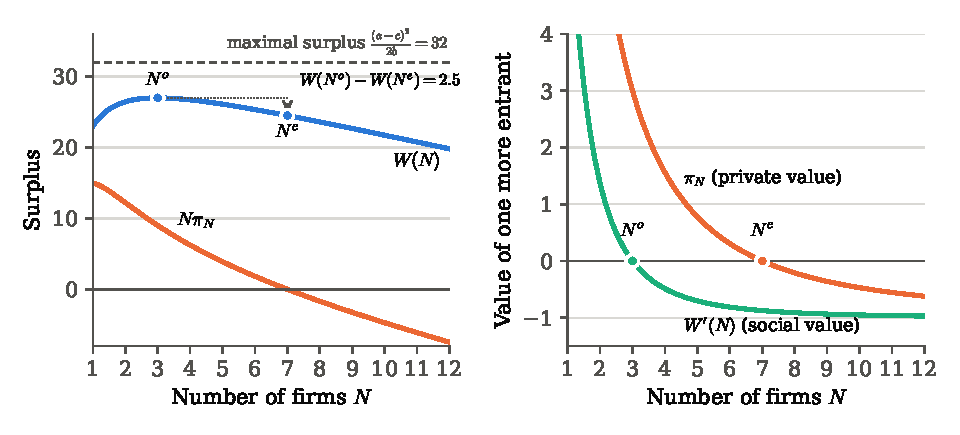
\includegraphics[width=\linewidth]{figures/ch02/entry_welfare.pdf}
\caption{Excess entry in the linear Cournot market with $a - c = 8$, $b = 1$ and $F = 1$. In the left panel, total
surplus $W(N)$ peaks at $N^o = 3$, while industry profit $N\pi_N$ reaches zero at $N^e = 7$. The welfare gap
$W(3) - W(7) = 27 - 24.5 = 2.5$ is 7.8 percent of the maximal surplus of 32. In the right panel, the private value
of entry $\pi_N$ exceeds its social value $W'(N)$ by the business-stealing term in \eqref{eq:02-mw-wprime}.}
\label{fig:02-entry}
\end{figure}

\begin{example}[Free entry into a cartel]\label{ex:02-mw-cartel}
Example~2 of \citet{MankiwWhinston1986} keeps the linear market but lets the entrants form a cartel. Total output is
the monopoly output $Q^m = \frac{a - c}{2b}$ for every $N$, and $q_N = \frac{Q^m}{N}$. Entry now steals business
one for one, since $N\frac{\dd q_N}{\dd N} = -\frac{Q^m}{N} = -q_N$. Using $P^m - c = \frac{a - c}{2}$ in
\eqref{eq:02-mw-wprime},
\begin{equation*}
W'(N) = \pi_N - (P^m - c)\, q_N = \left[(P^m - c)\, q_N - F\right] - (P^m - c)\, q_N = -F .
\end{equation*}
Each extra firm adds nothing but a set-up cost, so the optimum has one firm whenever the market should be served. Free
entry instead continues until $\pi_N = \frac{(a - c)^2}{4bN} - F = 0$, that is, until
$N^m = \frac{(a - c)^2}{4bF}$. Total set-up costs $N^m F = \frac{(a - c)^2}{4b}$ then equal the monopoly profit. The
whole monopoly rent is dissipated in duplicated set-up costs, as in the rent-seeking argument of
\citet{Posner1975} (see \cref{sec:02-welfare}). Welfare falls to the consumer surplus at the monopoly price,
$\frac{(a - c)^2}{8b}$, while one firm would give $\frac{3(a - c)^2}{8b} - F$. As $F \to 0$ the loss tends to
$\frac{(a - c)^2}{4b}$, half of the maximal surplus \citep[n.~10]{MankiwWhinston1986}.
\end{example}

\subsection{The integer constraint}\label{sec:02-mw-integer}

Treating $N$ as continuous is convenient but can mislead. In the cartel example, monopoly profit is
$\frac{(a - c)^2}{4b} - F$, and a monopoly is socially worth having when $\frac{3(a - c)^2}{8b} - F \ge 0$. When
$\frac{(a - c)^2}{4bF} \in [\frac{2}{3}, 1)$ the second condition holds and the first fails. No firm enters, although
one firm is optimal \citep[p.~53]{MankiwWhinston1986}. A monopolist captures only part of the surplus its entry
creates, so entry can be too low. With integers, the cartel example has excess entry only when
$\frac{(a - c)^2}{4bF} \ge 2$ \citep[n.~11]{MankiwWhinston1986}. The next result bounds the shortfall in general.

\begin{proposition}[At most one firm too few]\label{prop:02-mw-integer}
Suppose (E1) to (E3) of \cref{ass:02-mw} hold, with $N$ restricted to the integers and $N^o$ the integer maximizer of
$W$. Then $N^e \ge N^o - 1$ \citep[Proposition~2]{MankiwWhinston1986}.
\end{proposition}

\begin{proof}
The result is trivial when $N^o \le 1$, so let $N^o \ge 2$ and write $Q_N = N q_N$ and $n = N^o$. The proof follows
the appendix of \citet[p.~58]{MankiwWhinston1986}. It first shows that $\pi_{n - 1} \ge 0$ and then that $\pi_N$ is
nonincreasing in $N$.

\emph{Step 1.} Optimality of $n$ implies $W(n) \ge W(n - 1)$. By \eqref{eq:02-mw-welfare} this reads
\begin{equation*}
\int_{Q_{n-1}}^{Q_n} P(x)\, \dd x - n\, C(q_n) + (n - 1)\, C(q_{n-1}) \ge F .
\end{equation*}

\emph{Step 2.} Write $\pi_{n-1} = P(Q_{n-1})\, q_{n-1} - C(q_{n-1}) - F$ and replace $F$ by the larger quantity on
the left of Step~1:
\begin{equation*}
\pi_{n-1} \ge P(Q_{n-1})\, q_{n-1} - \int_{Q_{n-1}}^{Q_n} P(x)\, \dd x + n\left[C(q_n) - C(q_{n-1})\right].
\end{equation*}

\emph{Step 3.} Because $P$ is decreasing and $Q_n > Q_{n-1}$ by (E1), the integral is at most
$P(Q_{n-1})(Q_n - Q_{n-1})$. Moreover $q_{n-1} - (Q_n - Q_{n-1}) = n\, q_{n-1} - n\, q_n$. Hence
\begin{equation*}
\pi_{n-1} \ge n\, P(Q_{n-1})\left(q_{n-1} - q_n\right) + n\left[C(q_n) - C(q_{n-1})\right].
\end{equation*}

\emph{Step 4.} Convexity of $C$ gives, for any two outputs $q$ and $q'$,
\begin{equation}\label{eq:02-convex-ineq}
C(q') - C(q) \ge C'(q)\,(q' - q) .
\end{equation}
Applying it with $q = q_{n-1}$ and $q' = q_n$ yields
\begin{equation*}
\pi_{n-1} \ge n\left[P(Q_{n-1}) - C'(q_{n-1})\right]\left(q_{n-1} - q_n\right) \ge 0 ,
\end{equation*}
where the first factor is nonnegative by (E3) and the second is positive by (E2).

\emph{Step 5.} For any $N$, the fact that $P(Q_N) \le P(Q_{N-1})$ gives
\begin{align*}
\pi_N - \pi_{N-1} &= \left[P(Q_N)\, q_N - C(q_N)\right] - \left[P(Q_{N-1})\, q_{N-1} - C(q_{N-1})\right] \\
&\le P(Q_{N-1})\left(q_N - q_{N-1}\right) - \left[C(q_N) - C(q_{N-1})\right] \\
&\le \left[P(Q_{N-1}) - C'(q_{N-1})\right]\left(q_N - q_{N-1}\right) \le 0 ,
\end{align*}
using \eqref{eq:02-convex-ineq} in the third line and (E2), (E3) for the sign.

\emph{Step 6.} By \eqref{eq:02-free-entry}, $\pi_{N^e + 1} < 0$, and by Step~5 every $N \ge N^e + 1$ has negative
profit. Step~4 shows that $\pi_{n-1} \ge 0$, so $n - 1 < N^e + 1$. Since both sides are integers, $n - 1 \le N^e$.
\end{proof}

A shortfall of one firm can still be costly. In Example~3 of \citet{MankiwWhinston1986}, one firm in the linear market
acts as a monopolist, while two firms play Bertrand and price at $c$. A duopolist earns $-F$, so at most one firm
enters. A monopoly enters when $F \le \frac{(a - c)^2}{4b}$. Welfare is $W(1) = \frac{3(a - c)^2}{8b} - F$ with one
firm and $W(2) = \frac{(a - c)^2}{2b} - 2F$ with two. Duopoly is better when $F \le \frac{(a - c)^2}{8b}$. The loss
from one firm too few is then $\frac{(a - c)^2}{8b} - F$, which approaches 25 percent of the maximal surplus as
$F \to 0$ \citep[pp.~53--54]{MankiwWhinston1986}. Business stealing holds here only weakly, since
$q_1 = q_2 = \frac{a - c}{2b}$.

\subsection{Product diversity}\label{sec:02-diversity}

With differentiated products a new entrant also adds variety. Following \citet{Spence1976},
\citet[pp.~54--55]{MankiwWhinston1986} write gross consumer benefit as $G\left(\sum_i \psi(q_i)\right)$, where
$q_i$ is firm $i$'s output. The subutility $\psi$ satisfies $\psi(0) = 0$, $\psi' > 0$ and $\psi'' \le 0$, and $G$
satisfies $G' > 0$ and $G'' < 0$. These assumptions say that consumers like variety and that the products are
substitutes. (The symbols $G$ and $\psi$ are local to this subsection.) With $N$ symmetric firms the planner solves
\begin{equation}\label{eq:02-diversity-W}
\max_N\; W(N) = G\left(N \psi(q_N)\right) - N C(q_N) - N F .
\end{equation}
Consumer optimization sets each firm's price equal to the marginal benefit of its output,
$p_N = G'\left(N\psi(q_N)\right)\psi'(q_N)$, so per-firm profit is
\begin{equation*}
\pi_N = G'\left(N\psi(q_N)\right)\psi'(q_N)\, q_N - C(q_N) - F .
\end{equation*}
Differentiating \eqref{eq:02-diversity-W}, with arguments suppressed, gives
\begin{equation*}
W'(N) = G'\left[N\psi'\frac{\dd q_N}{\dd N} + \psi\right] - C(q_N) - N C'\frac{\dd q_N}{\dd N} - F .
\end{equation*}
Adding and subtracting $G'\psi' q_N$ and regrouping yields the generalization of \eqref{eq:02-mw-wprime}:
\begin{equation}\label{eq:02-diversity-wprime}
W'(N) = \pi_N + N\left[G'\psi' - C'\right]\frac{\dd q_N}{\dd N} + G'\left[\psi(q_N) - \psi'(q_N)\, q_N\right] .
\end{equation}
The second term is the business-stealing wedge, now with price $G'\psi'$. It is negative when price exceeds marginal
cost and entry contracts incumbents. The third term is new. $G'\psi$ is the entrant's contribution to gross surplus,
while $G'\psi' q_N$ is its revenue. Concavity and $\psi(0) = 0$ imply $\psi(q) \ge \psi'(q)\, q$, so the third term is
nonnegative. It is the surplus from added variety that the entrant cannot appropriate. In the homogeneous case
$\psi(q) = q$ and $G(Q) = \int_0^Q P(x)\,\dd x$, the third term vanishes and \eqref{eq:02-mw-wprime} returns.

The two wedges push in opposite directions, so the sign of the entry bias is ambiguous. With $\psi(q) = q^{\varsigma}$
for some $\varsigma < 1$ and firms that take $G'$ as given, the diversity term dominates for every $N$ and entry is
too low \citep{Spence1976}. \citet{DixitStiglitz1977} also show that monopolistic
competition can produce too little entry. Replacing Spence's price taking with conjectural variations can reverse
this result \citep{KoenkerPerry1981}. \citet[p.~55]{MankiwWhinston1986} also give a functional form, with a quadratic
$\psi$ and linear cost, in which business stealing dominates and entry is excessive. Demand substitutability is
neither necessary nor sufficient for business stealing \citep[n.~14]{MankiwWhinston1986}. Spatial models give further
examples. In the circular city with linear transport costs, the free-entry number of firms is twice the optimum
\citep[sec.~7.1.2]{Tirole1988}, and \cref{ch:diffprod} develops these location models.

\subsection{Small set-up costs}\label{sec:02-small-F}

\Cref{tab:02-mw} shows the loss from excess entry falling as set-up costs fall. The cartel example shows that this
need not happen. There the loss tends to half of the maximal surplus as $F \to 0$. Mankiw and Whinston isolate what
separates the two cases. Write $W^o_F$ and $W^e_F$ for welfare at the optimum and under free entry when the set-up
cost is $F$, and $p_N = G'\left(N\psi(q_N)\right)\psi'(q_N)$ for the price.

\begin{proposition}[Vanishing loss as set-up costs vanish]\label{prop:02-mw-small}
Suppose (E2) holds and, in addition, (i) $p_N$ is decreasing in $N$ and $\lim_{N\to\infty} N\psi(q_N) < \infty$,
(ii) $p_N - C'(q_N) > 0$ for all $N$, and (iii) $\lim_{N\to\infty}\left[p_N - C'(q_N)\right] = 0$. Then
$\lim_{F\to 0}\left(W^o_F - W^e_F\right) = 0$ \citep[Proposition~3]{MankiwWhinston1986}.
\end{proposition}

\begin{proof}[Proof sketch]
Let $W^\infty = \lim_{N\to\infty}\left[G\left(N\psi(q_N)\right) - N C(q_N)\right]$. This limit is finite and is the
best welfare attainable with no set-up cost, so $W^\infty \ge W^o_F \ge W^e_F$ for every $F$. It suffices to show
that $W^e_F \to W^\infty$. First, $N^e_F \to \infty$ as $F \to 0$. Otherwise, for small enough $F$ one more firm
would earn $(p_N - \frac{C(q_N)}{q_N})\, q_N - F \ge (p_N - C'(q_N))\, q_N - F > 0$, using $C(q) \le C'(q)\, q$ for
convex $C$ with $C(0) = 0$. Given $N^e_F \to \infty$, welfare under free entry converges to $W^\infty$ exactly when
total set-up costs $N^e_F F$ vanish. The zero-profit condition bounds them:
\begin{equation*}
N^e F \le \left[p_{N^e} - \frac{C(q_{N^e})}{q_{N^e}}\right] N^e q_{N^e} .
\end{equation*}
As $N^e \to \infty$, per-firm output tends to zero because $N\psi(q_N)$ stays bounded. Average cost and marginal cost
then both tend to $C'(0)$, so the bracket tends to $\lim\left[p_N - C'(q_N)\right] = 0$ by (iii). Total output
$N^e q_{N^e}$ stays bounded, so $N^e F \to 0$.
\end{proof}

Two assumptions do the work. Price must exceed marginal cost for every finite $N$, which is (ii), and approach it
as $N$ grows, which is (iii). Mankiw and Whinston assume both and leave the post-entry game unspecified.
\citet{Novshek1980} derives (iii) for Cournot competition as efficient scale shrinks. Linear Cournot satisfies
(ii) and (iii), which is why the losses in \cref{tab:02-mw} decline. The cartel example violates (iii), since price
stays at the monopoly level for every $N$. Example~3 satisfies (iii) but violates (ii). Price falls to marginal
cost already at $N = 2$, so a second entrant cannot cover its set-up cost. The loss from having one firm too few
therefore persists as $F \to 0$ \citep[p.~57]{MankiwWhinston1986}. The upshot is that regulating entry matters most in markets
with large set-up costs and imperfect competition. It matters little where entry is cheap and competition is close
to perfect.

\subsection{Margins and concentration under fixed and free entry}\label{sec:02-LH}

Free entry changes how margins and concentration move together. With a fixed number of firms, concentration is a
primitive and the Lerner index responds to it. With free entry, both are equilibrium outcomes driven by the same
primitives. The linear market makes the point precisely, using the four columns of \cref{tab:02-linear-cournot}.

\begin{example}[Lerner index and Herfindahl index in four regimes]\label{ex:02-LH}
Let $P = a - bQ$, marginal cost $c$, set-up cost $F$, and $r \equiv \sqrt{bF}$.

\emph{Cournot with fixed $N$.} Here $L = \frac{a - c}{a + Nc}$ and $\HHI = \frac{1}{N}$. Substituting
$N = \frac{1}{\HHI}$ and multiplying numerator and denominator by $\HHI$,
\begin{equation}\label{eq:02-LH-cournot}
L = \frac{(a - c)\,\HHI}{a\,\HHI + c}, \qquad
\frac{\dd L}{\dd \HHI} = \frac{c(a - c)}{(a\,\HHI + c)^2} > 0, \qquad
\frac{\dd^2 L}{\dd \HHI^2} = -\frac{2ac(a - c)}{(a\,\HHI + c)^3} < 0 .
\end{equation}
The relation is increasing and concave. It is causal, since $N$ is set from outside.

\emph{Cournot with free entry.} From \cref{ex:02-free-entry-linear}, $L = \frac{r}{c + r}$ and
$\HHI = \frac{r}{a - c - r}$. These points lie on the curve \eqref{eq:02-LH-cournot} for the same $(a, c)$, because
\begin{equation*}
\frac{(a - c)\frac{r}{a - c - r}}{\frac{a\, r}{a - c - r} + c} = \frac{(a - c)\, r}{a\, r + c(a - c - r)}
= \frac{(a - c)\, r}{(a - c)(r + c)} = \frac{r}{c + r} .
\end{equation*}
Both indices are now endogenous. A higher $F$ or $b$ raises $r$ and moves the industry up along the curve. A higher
$a$ lowers $\HHI$ and leaves $L$ unchanged. A higher $c$ lowers $L$ and raises $\HHI$.

\emph{Collusion with fixed $N$.} Here $L = \frac{a - c}{a + c}$ for every $N$, while $\HHI = \frac{1}{N}$. The
Lerner index does not depend on concentration at all.

\emph{Collusion with free entry.} By \cref{ex:02-mw-cartel}, $N^m = \frac{(a - c)^2}{4bF}$, so
$\HHI = \frac{4bF}{(a - c)^2}$ and $L = \frac{a - c}{a + c}$. A higher $F$ or $b$ raises $\HHI$ only. A higher $a$
raises $L$ and lowers $\HHI$, and a higher $c$ does the reverse.

Finally, collusion attracts more entrants than Cournot competition. With $x = \frac{a - c}{\sqrt{bF}}$,
\eqref{eq:02-Ne-linear} gives $N^e = x - 1$, while $N^m = \frac{x^2}{4}$. Then
\begin{equation*}
N^m - N^e = \frac{x^2}{4} - x + 1 = \left(\frac{x}{2} - 1\right)^2 \ge 0 .
\end{equation*}
\end{example}

\begin{table}[htbp]
\centering
\begin{threeparttable}
\caption{Comparative statics of the Lerner and Herfindahl indices in the linear market}
\label{tab:02-LH-cases}
\renewcommand{\arraystretch}{1.6}
\begin{tabular}{@{}lcccccc@{}}
\toprule
 & & & \multicolumn{4}{c}{Effect of a higher primitive on $(L, \HHI)$} \\
\cmidrule(l){4-7}
Regime & $L$ & $\HHI$ & $F$ & $b$ & $a$ & $c$ \\
\midrule
Cournot, fixed $N$ & $\frac{a - c}{a + Nc}$ & $\frac{1}{N}$ & $(0, 0)$ & $(0, 0)$ & $(+, 0)$ & $(-, 0)$ \\
Cournot, free entry & $\frac{\sqrt{bF}}{c + \sqrt{bF}}$ & $\frac{\sqrt{bF}}{a - c - \sqrt{bF}}$ & $(+, +)$ &
  $(+, +)$ & $(0, -)$ & $(-, +)$ \\
Collusion, fixed $N$ & $\frac{a - c}{a + c}$ & $\frac{1}{N}$ & $(0, 0)$ & $(0, 0)$ & $(+, 0)$ & $(-, 0)$ \\
Collusion, free entry & $\frac{a - c}{a + c}$ & $\frac{4bF}{(a - c)^2}$ & $(0, +)$ & $(0, +)$ & $(+, -)$ &
  $(-, +)$ \\
\bottomrule
\end{tabular}
\begin{tablenotes}\footnotesize
\item Notes: $P = a - bQ$, constant marginal cost $c$, set-up cost $F$. Each cell gives the signs of the effects on
$L$ and $\HHI$. Under free entry the number of firms is treated as continuous.
\end{tablenotes}
\end{threeparttable}
\end{table}

\begin{figure}[htbp]
\centering
\begin{tikzpicture}
\begin{axis}[
  width=0.86\linewidth, height=0.62\linewidth,
  xmin=0, xmax=1.02, ymin=0.25, ymax=0.78,
  xlabel={Herfindahl index $\HHI$}, ylabel={Lerner index $L$},
  xtick={0,0.25,0.5,0.75,1}, ytick={0.3,0.4,0.5,0.6,0.7},
  axis lines=left, every axis plot/.append style={thick},
  clip=false]
  \addplot[domain=0.1:1, samples=120, blue!70!black] {8*x/(10*x+2)};
  \node[blue!70!black, anchor=north west, font=\small, align=left] at (axis cs:0.62,0.585)
    {Cournot\\ $a = 10$, $c = 2$};
  \addplot[domain=0.075:1, samples=120, blue!70!black, dashed, thin] {10*x/(12*x+2)};
  \node[blue!70!black, anchor=west, font=\footnotesize] at (axis cs:1.0,0.725) {$a = 12$};
  \addplot[domain=0.17:1, samples=120, blue!70!black, dotted, thin] {7*x/(10*x+3)};
  \node[blue!70!black, anchor=west, font=\footnotesize] at (axis cs:1.0,0.538) {$c = 3$};
  \addplot[domain=0:1, samples=2, orange!85!black] {2/3};
  \node[orange!85!black, anchor=south west, font=\small] at (axis cs:0.40,0.672)
    {collusion, $L = \frac{a - c}{a + c}$};
  \addplot[only marks, mark=*, mark size=2pt, black] coordinates {(0.3333,0.5)};
  \node[anchor=north, font=\footnotesize] at (axis cs:0.3333,0.488) {$A$};
  \draw[-{Stealth[length=2.2mm]}, thick] (axis cs:0.3333,0.5) -- (axis cs:0.4545,0.5556);
  \node[anchor=north west, font=\footnotesize] at (axis cs:0.462,0.545) {$F$ or $b$ up};
  \draw[-{Stealth[length=2.2mm]}, thick] (axis cs:0.3333,0.5) -- (axis cs:0.25,0.5);
  \draw[thin, gray] (axis cs:0.245,0.503) -- (axis cs:0.16,0.56);
  \node[anchor=south, font=\footnotesize] at (axis cs:0.15,0.56) {$a$ up};
  \draw[-{Stealth[length=2.2mm]}, thick] (axis cs:0.3333,0.5) -- (axis cs:0.4,0.4);
  \node[anchor=north west, font=\footnotesize] at (axis cs:0.40,0.40) {$c$ up};
  \addplot[only marks, mark=square*, mark size=2pt, orange!85!black] coordinates {(0.25,0.6667)};
  \draw[densely dashed, gray] (axis cs:0.3333,0.5) -- (axis cs:0.25,0.6667);
  \node[anchor=south east, font=\footnotesize] at (axis cs:0.25,0.6667) {$B$};
\end{axis}
\end{tikzpicture}
\caption{Lerner index against Herfindahl index in the linear market with $a = 10$, $c = 2$, $b = 1$. The solid curve
is $L = \frac{8\,\HHI}{10\,\HHI + 2}$, the Cournot relation \eqref{eq:02-LH-cournot}. Point $A$ is the Cournot
free-entry outcome with $F = 4$ ($N^e = 3$). Arrows show the free-entry responses to higher $F$ or $b$ (along the
curve), higher $a$ (onto the dashed curve) and higher $c$ (onto the dotted curve). Point $B$ is the collusive
free-entry outcome with the same primitives ($N^m = 4$). It has a higher margin and lower concentration than $A$.}
\label{fig:02-LH}
\end{figure}

The lesson is a theoretical one. The sign of a cross-industry relation between margins and concentration depends on
which primitive varies across industries and on how firms compete. Points $A$ and $B$ in \cref{fig:02-LH} share every
primitive and differ only in conduct. A sample that mixes Cournot and collusive industries pairs high margins with low
concentration and can produce a flat or negative slope. A regression of $L$ on $\HHI$ across industries therefore has
no structural interpretation without a model of entry and conduct. \Cref{ch:intro} discusses these regressions, and
\cref{app:problems} works through the full problem.

\section{Bertrand competition and capacity constraints}\label{sec:02-bertrand}

Cournot firms choose quantities and let the market set the price. Many firms instead post prices and serve whatever
demand arrives. This section studies price competition with a homogeneous good. Its main result is stark: two firms
suffice for the competitive price. We then show how capacity constraints undo the result and when quantity
competition is the better description.

\subsection{Price competition with a homogeneous good}\label{sec:02-bertrand-homog}

\begin{definition}[Bertrand game with a homogeneous good]\label{def:02-bertrand}
There are $N \ge 2$ firms with constant marginal costs $c_i$ and no capacity limits. Market demand $Q(p)$ is
continuous and nonincreasing. Firms choose prices $p_i \ge 0$ simultaneously. Let $p_{\min} = \min_i p_i$ and let
$k$ be the number of firms that charge $p_{\min}$. Each of these firms sells $\frac{Q(p_{\min})}{k}$, and every other
firm sells nothing. Firm $i$ earns $(p_i - c_i)\, q_i$, and each firm must serve all demand at its posted price.
\end{definition}

These are the stage-game rules used for repeated price competition in \cref{ch:collusion-theory}. In the static game
with symmetric costs the tie rule (equal split) does not affect equilibrium outcomes. It matters with asymmetric
costs and for the collusive shares in the repeated game.

\begin{proposition}[The Bertrand paradox]\label{prop:02-bertrand}
Suppose all firms have the same marginal cost $c$ and $Q(c) > 0$. Then a pure-strategy Nash equilibrium exists. In
every pure-strategy Nash equilibrium $p_{\min} = c$, at least two firms charge $c$, and every firm earns zero profit.
\end{proposition}

\begin{proof}
Take any price profile and consider four exhaustive cases.

\emph{Case 1, $p_{\min} < c$.} The firms charging $p_{\min}$ sell $\frac{Q(p_{\min})}{k} \ge \frac{Q(c)}{k} > 0$ at a
loss. Any of them can raise its price above $p_{\min}$ and sell nothing, earning zero. So the profile is not an
equilibrium.

\emph{Case 2, $p_{\min} > c$ and $Q(p_{\min}) > 0$.} If $k \ge 2$, a firm at $p_{\min}$ earns
$(p_{\min} - c)\frac{Q(p_{\min})}{k}$. By cutting its price to $p_{\min} - \eta$ it serves the whole market and earns
at least $(p_{\min} - \eta - c)\, Q(p_{\min})$, because $Q$ is nonincreasing. For small $\eta > 0$ this exceeds its
current profit, since $k \ge 2$. If $k = 1$, any other firm earns zero and can charge a price $p' \in (c, p_{\min})$,
earning $(p' - c)\, Q(p') \ge (p' - c)\, Q(p_{\min}) > 0$. Either way someone deviates.

\emph{Case 3, $p_{\min} > c$ and $Q(p_{\min}) = 0$.} Every firm earns zero. By continuity of $Q$ and $Q(c) > 0$ there
is a price $p'$ slightly above $c$ with $Q(p') > 0$, and $p' < p_{\min}$ because $Q$ is nonincreasing. A firm that
deviates to $p'$ earns $(p' - c)\, Q(p') > 0$.

\emph{Case 4, $p_{\min} = c$.} If only one firm charges $c$, it earns zero. Let $p_{(2)} > c$ be the second-lowest
price. By continuity it can raise its price to some $p' \in (c, p_{(2)})$ with $Q(p') > 0$ and earn a positive
profit. So at least two firms must charge $c$. In that case every firm earns zero. A firm that raises its price sells
nothing and still earns zero, and a firm that cuts below $c$ makes a loss. No deviation is profitable, so any profile
with at least two firms at $c$ is an equilibrium.
\end{proof}

The paradox is the contrast with \cref{sec:02-cournot}. A symmetric Cournot duopoly has industry conduct
$\theta = \frac{1}{2}$ (\cref{sec:02-conduct}). A Bertrand duopoly prices at
marginal cost, so $\theta = 0$ even with two firms. The number of firms alone does not pin down margins. The mode of
competition matters just as much. Two firms suffice for competitive pricing only under stark assumptions: identical
products, constant marginal cost, no capacity limits, and a single round of play. Each assumption points to a
resolution. Capacity constraints are the subject of \cref{sec:02-capacity}. Product differentiation is the subject of
\cref{ch:diffprod}. Repeated interaction is previewed in \cref{sec:02-collusion} and developed in
\cref{ch:collusion-theory}.

\casehead{Asymmetric costs} Let $c_1 < c_2 \le c_j$ for all $j \ge 3$, and let $p^m(c_1)$ be the monopoly price of a
firm with cost $c_1$. If $p^m(c_1) \le c_2$, firm 1's cost advantage is \emph{drastic}. It charges $p^m(c_1)$ and
serves the market, while rivals price at or above their costs. If $p^m(c_1) > c_2$, firm 1 wants to price just below
$c_2$. With continuous prices and an equal split of ties, there is no largest price below $c_2$, so a pure
equilibrium fails to exist. Two standard modifications restore one. If ties go to the low-cost firm, then
$p_1 = p_2 = c_2$ is an equilibrium in which firm 1 serves the market and earns $(c_2 - c_1)\, Q(c_2)$. If prices lie
on a grid with step $\iota$ and $c_2$ on the grid, then $p_1 = c_2$ and $p_2 = c_2 + \iota$ is an equilibrium for
small $\iota$. In this equilibrium firm 2 avoids the weakly dominated choice of pricing at its own cost. Either way, the market price
is
\begin{equation*}
P = \min\left\{c_2,\; p^m(c_1)\right\}.
\end{equation*}
The efficient firm earns a margin limited by its rival's cost, with Lerner index $\frac{c_2 - c_1}{c_2}$ in the
non-drastic case. Measured against the producing firm's marginal cost $c_1$, this market shows a positive conduct
parameter $\theta = \varepsilon\frac{c_2 - c_1}{c_2}$, although firms play Bertrand. A positive estimated $\theta$ can
thus reflect cost asymmetry as well as softer conduct.

\begin{remark}[Increasing marginal cost]\label{rem:02-bertrand-convex}
Let $N$ symmetric firms have a strictly convex cost $C(q)$ with $C(0) = 0$, and keep the obligation to serve all
demand at the posted price. Consider a common price $p$ at which each firm sells $\frac{Q(p)}{N}$ and earns
$u(p) = \frac{p\, Q(p)}{N} - C\left(\frac{Q(p)}{N}\right)$. Raising the price sells nothing and earns $C(0) = 0$.
Undercutting slightly serves the whole market and earns close to $v(p) = p\, Q(p) - C(Q(p))$. For prices below the
level that maximizes $v$, the common price $p$ is an equilibrium if and only if
\begin{equation*}
u(p) \ge 0 \qquad\text{and}\qquad u(p) \ge v(p) .
\end{equation*}
Both conditions hold strictly at the competitive price $p^*$, defined by $p^* = C'\left(\frac{Q(p^*)}{N}\right)$.
Write $q^* = \frac{Q(p^*)}{N}$. The first holds because average cost is below marginal cost for strictly convex $C$
with $C(0) = 0$. For the second, apply \eqref{eq:02-convex-ineq} strictly:
\begin{equation*}
v(p^*) - u(p^*) = p^*\left(Nq^* - q^*\right) - \left[C(Nq^*) - C(q^*)\right]
< p^*\left(Nq^* - q^*\right) - C'(q^*)\left(Nq^* - q^*\right) = 0 .
\end{equation*}
By continuity both inequalities also hold in an interval of prices around $p^*$. Pure equilibria therefore exist and
form a continuum, with prices above and below the competitive level \citep{Dastidar1995}.

Without the obligation to serve, a firm sells only what it wishes at its posted price. Firm $i$'s \emph{competitive
supply} $S_i(p)$ is defined by $p = C_i'(S_i(p))$, and a firm never sells more than $S_i(p)$. The natural candidate is
then the competitive price $p^*$, with $S_1(p^*) + S_2(p^*) = Q(p^*)$ in a duopoly. Suppose rationing is
\emph{efficient}, so that the consumers with the highest willingness to pay are served first (\cref{def:02-rationing}
below). Then $p^*$ is not an equilibrium \citep[sec.~5.3.2]{Tirole1988}. Let firm 2 charge $p^*$ and sell
$q_2^* = S_2(p^*)$, and write $q_1^* = S_1(p^*)$. If firm 1 raises its price to some $p$ slightly above $p^*$, it
serves the residual demand $Q(p) - q_2^*$, which is below $S_1(p)$. Its profit is
$p\,[Q(p) - q_2^*] - C_1(Q(p) - q_2^*)$, whose derivative at $p^*$ is
\begin{equation*}
Q(p^*) - q_2^* + \bigl[p^* - C_1'(q_1^*)\bigr]Q'(p^*) = q_1^* > 0 ,
\end{equation*}
because $Q(p^*) - q_2^* = q_1^*$ and $p^* = C_1'(q_1^*)$. The units lost were sold at marginal cost, so the loss is of
second order, while the higher price on the remaining units is a first-order gain. Equilibria then generally involve
mixed strategies, and both firms' prices exceed the competitive price. Decreasing returns therefore soften price
competition, and the capacity constraint of \cref{sec:02-capacity} is the extreme case.
\end{remark}

\begin{remark}[Strategic substitutes and complements]\label{rem:02-strategic}
\citet[p.~489]{BulowGeanakoplosKlemperer1985} call a lower price or a higher quantity a ``more aggressive'' move.
They classify competition by how a rival's aggressive move changes the \emph{marginal} profit of the firm's own
aggressive move. Choices are strategic substitutes when the rival's aggressive move lowers this marginal profit and
\emph{strategic complements} when it raises it.
Equivalently, best responses slope down under substitutes and up under complements. \Cref{sec:02-cournot-br}
showed that quantities are substitutes in Cournot competition under \cref{ass:02-cournot}. With differentiated products and linear demand
$q_i = d_0 - d_1 p_i + d_2 p_j$, where $0 < d_2 < d_1$, profit $(p_i - c)\, q_i$ gives
$\frac{\partial^2 \pi_i}{\partial p_i \partial p_j} = d_2 > 0$. A lower $p_j$ therefore lowers
$\frac{\partial \pi_i}{\partial p_i}$, which raises the marginal profit of cutting $p_i$. Prices are complements, and
the best response $p_i = \frac{d_0 + d_1 c + d_2 p_j}{2 d_1}$ slopes up, with slope
$\frac{d_2}{2d_1} \in \left(0, \frac{1}{2}\right)$ as \eqref{eq:02-reaction-slope} predicts. \citet[sec.~11.2]{Tirole1988}
uses the same linear demand, $q_i = 1 - bp_i + dp_j$, to illustrate Nash equilibrium in prices. The classification
depends on demand as well as on the strategic variable. \citet[p.~490]{BulowGeanakoplosKlemperer1985} note that
Cournot competition with constant-elasticity demand may yield strategic complements. Our derivation from
\cref{rem:02-c2} gives the threshold. With constant-elasticity demand, $P' + q_i P'' = P'\left(1 - s_i \chi\right)$ with
curvature $\chi = 1 + \frac{1}{\varepsilon}$. The cross-partial is therefore positive, and quantities are complements,
when $s_i\left(1 + \frac{1}{\varepsilon}\right) > 1$.
\end{remark}

\subsection{Capacity constraints and rationing}\label{sec:02-capacity}

\citet{Edgeworth1925}, in an article first published in Italian in 1897, observed that the Bertrand outcome collapses
once firms cannot serve the whole market \citep[sec.~5.2.1]{Tirole1988}. Let two
firms have constant marginal cost $c$ up to capacities $k_1$ and $k_2$, beyond which they cannot produce. Suppose
$k_2 < Q(c)$ and both firms charge $c$. If firm 1 raises its price slightly, firm 2 cannot serve everyone who wants to
buy at $c$. Some consumers turn to firm 1 at the higher price, and firm 1 earns a positive margin on them. So
$p_1 = p_2 = c$ is no longer an equilibrium. When capacities are intermediate, no pure-strategy equilibrium exists at
all. Firms undercut each other until one prefers to raise its price and serve the leftover demand, and the cycle
repeats. The equilibrium of the static game is in mixed strategies \citep{LevitanShubik1972}. What a high-price firm
can sell depends on which consumers the low-price firm serves.

\begin{definition}[Rationing rules]\label{def:02-rationing}
Let firm 1 charge $p_1 < p_2$ with capacity $k_1 < Q(p_1)$. A \emph{rationing rule} gives the residual demand
$Q_2(p_2)$ left for firm 2.
\begin{enumerate}[label=(\roman*)]
\item Under \emph{efficient rationing}, firm 1 serves the consumers with the highest willingness to pay first. Firm 2
  faces
  \begin{equation*}
  Q_2(p_2) = \max\left\{0,\; Q(p_2) - k_1\right\}.
  \end{equation*}
\item Under \emph{proportional rationing}, every consumer who wants to buy at $p_1$ is equally likely to be served
  by firm 1. The fraction $\frac{k_1}{Q(p_1)}$ of them is served. The unserved consumers are a random sample, so a
  fraction $1 - \frac{k_1}{Q(p_1)}$ of the demand at any price remains:
  \begin{equation*}
  Q_2(p_2) = Q(p_2)\left(1 - \frac{k_1}{Q(p_1)}\right).
  \end{equation*}
\end{enumerate}
\end{definition}

Efficient rationing maximizes consumer surplus given the capacities, since the units go to those who value them most.
It also leaves the high-price firm the least demand. Proportional residual demand is larger because
\begin{equation*}
Q(p_2)\left(1 - \frac{k_1}{Q(p_1)}\right) \ge Q(p_2) - k_1
\quad\Longleftrightarrow\quad
\frac{Q(p_2)}{Q(p_1)}\, k_1 \le k_1 ,
\end{equation*}
which holds because $Q(p_2) \le Q(p_1)$. \Cref{fig:02-rationing} draws both residual demands. Efficient rationing
shifts demand inward in parallel by $k_1$. Proportional rationing rotates it around the choke price.

\citet[sec.~5.3.1]{Tirole1988} interprets the two rules. Efficient rationing is the outcome if consumers can resell the
good to each other at no cost, since such arbitrage moves the units to those who value them most. It also arises when
identical consumers with downward-sloping demands are each rationed equally. Proportional rationing, also called
randomized rationing, gives every consumer the same chance of being served. It leaves some low-value consumers with the
bargain, and the high-price firm prefers it because its residual demand is larger. Many other rules are possible.
Suppose rationing works through queues, and the most eager buyers also have the highest value of time. Then the least
eager buyers may end up with the low price. In applications the rationing rule stands in for a model of consumer
behavior, and the right rule depends on the market.

\begin{figure}[htbp]
\centering
\begin{tikzpicture}[scale=0.62, >=Stealth]
  \draw[->] (0,0) -- (10.2,0) node[below] {$q$};
  \draw[->] (0,0) -- (0,10.2) node[left] {$p$};
  \draw[very thick, black] (0,9) -- (9,0) node[pos=0.85, above right] {$Q(p)$};
  \node[below] at (9,0) {$Q(0)$};
  \draw[dashed, gray] (0,3) -- (6,3);
  \node[left] at (0,3) {$p_1$};
  \draw[very thick, orange!85!black] (0,3) -- (3,3);
  \draw[decorate, decoration={brace, amplitude=5pt, mirror}] (0,2.8) -- (3,2.8)
    node[midway, below=5pt] {$k_1$};
  \draw[dotted] (6,3) -- (6,0) node[below] {$Q(p_1)$};
  \draw[very thick, blue!70!black] (3,3) -- (0,6);
  \draw[very thick, blue!70!black, dashed] (3,3) -- (0,9);
  \node[blue!70!black, anchor=west, font=\small] (eff) at (6.2,6.4) {$Q(p) - k_1$ (efficient)};
  \draw[thin, gray] (eff.west) -- (1.0,5.0);
  \node[blue!70!black, anchor=west, font=\small] (prop) at (5.2,8.6)
    {$Q(p)\left(1 - \frac{k_1}{Q(p_1)}\right)$ (proportional)};
  \draw[thin, gray] (prop.west) -- (1.2,6.6);
  \fill (3,3) circle (2.5pt);
  \node[anchor=north west, font=\small] at (3,2.9) {$Q(p_1) - k_1$};
  \node[left] at (0,9) {$\bar p$};
  \node[left] at (0,6) {$P(k_1)$};
\end{tikzpicture}
\caption{Residual demand of the high-price firm. Firm 1 charges $p_1$ and sells its capacity $k_1 < Q(p_1)$. Under
efficient rationing firm 2 faces $Q(p) - k_1$ for $p > p_1$ (solid), a parallel inward shift of demand. Under
proportional rationing it faces $Q(p)\left(1 - \frac{k_1}{Q(p_1)}\right)$ (dashed), which rotates demand around the
choke price $\bar p$. Drawn for $Q(p) = 9 - p$, $p_1 = 3$ and $k_1 = 3$.}
\label{fig:02-rationing}
\end{figure}

\citet{KrepsScheinkman1983} turn Edgeworth's problem into a foundation for Cournot competition. Firms first choose
capacities and then, having observed them, compete in prices. Write $r_\gamma(k)$ for the Cournot best response of a
firm with constant marginal cost $\gamma$ to rival output $k$.

\begin{proposition}[Capacity commitment yields Cournot outcomes]\label{prop:02-ks}
Consider a duopoly in which firms first build capacities $k_i$ at constant unit cost $c_k > 0$, then observe them
and set prices. Production costs $c \ge 0$ per unit up to capacity. Suppose inverse demand is concave and residual
demand follows efficient rationing. Then the game has a unique subgame-perfect equilibrium outcome. It coincides with
the Cournot outcome of the one-stage game with marginal cost $c + c_k$ \citep{KrepsScheinkman1983}.
\end{proposition}

A linear example shows the mechanism before the general argument \citep[sec.~5.3.2.1]{Tirole1988}.

\begin{example}[Capacity-constrained price competition with linear demand]\label{ex:02-ks-linear}
Let $Q(p) = 1 - p$, let capacity cost $c_k \in \left[\frac{3}{4}, 1\right]$ per unit, and let production cost nothing
up to capacity. Rationing is efficient. No firm builds more than $\frac{1}{3}$. In the pricing stage a firm cannot
earn more than the monopoly revenue $\max_p p(1 - p) = \frac{1}{4}$. Its net profit is therefore at most
$\frac{1}{4} - c_kk_i$, which is negative for $k_i > \frac{1}{3}$ because $c_k \ge \frac{3}{4}$.

Take capacities in $\left[0, \frac{1}{3}\right]$. We claim that both firms charging the market-clearing price
$p^* = 1 - k_1 - k_2$ is an equilibrium of the pricing stage. A lower price gains nothing, since firm $i$ already
sells its whole capacity at $p^*$. At a higher price $p > p^*$, firm $i$ sells the residual demand
$q = 1 - p - k_j < k_i$. Its revenue $pq$ is then $(1 - q - k_j)q$, the Cournot objective against rival output
$k_j$. This objective is concave in $q$, and its derivative at $q = k_i$ is $1 - 2k_i - k_j \ge 0$. Revenue therefore
rises on $[0, k_i]$, and the best choice is $q = k_i$, that is, the price $p^*$. The reduced-form profits after the
pricing stage are
\begin{equation}\label{eq:02-ks-linear}
  \Pi_i(k_i, k_j) = (1 - k_i - k_j)\,k_i - c_k k_i ,
\end{equation}
the profits net of capacity cost. This is Tirole's eq.~(5.3). His eq.~(5.2) is the same profit gross of capacity
cost, $(1 - k_i - k_j)k_i$. The net profits are exactly the Cournot profits for outputs $k_i$ and marginal cost
$c_k$. The capacity stage is therefore a Cournot game. Its equilibrium has $k_1 = k_2 = \frac{1 - c_k}{3} \le
\frac{1}{12}$ and price $p^* = \frac{1 + 2c_k}{3}$.
\end{example}

\casehead{Two foundations for Cournot} \citet[sec.~5.3.4]{Tirole1988} separates two results. The pricing stage has
an \emph{exact Cournot reduced form} when, at every pair of capacities that can arise, its equilibrium profits equal
the Cournot profits with quantities read as capacities. The two-stage game has a \emph{Cournot outcome} when its
subgame-perfect capacities and price coincide with the Cournot equilibrium. The first result implies the second,
because the capacity stage is then the Cournot game. It also covers variants, such as capacities chosen in sequence.
\Cref{ex:02-ks-linear} has the exact reduced form. \Cref{prop:02-ks} claims only the Cournot outcome. In its general
setting the reduced form is Cournot for small capacities only, and large capacities lead to mixed equilibria with
other payoffs.

\casehead{The pricing stage} To simplify, set the production cost to $c = 0$, as \citet[sec.~5.7.2.1]{Tirole1988}
does, and assume $k_1 + k_2 < Q(0)$. Write $r(k) = r_0(k)$ for the output that maximizes $qP(q + k)$. Inverse demand
is concave, so this objective is strictly concave in $q$. By \cref{lem:02-cournot-br}, $r$ is single-valued and
decreasing, with slope in $(-1, 0)$.

\begin{lemma}[Pure equilibria clear the market]\label{lem:02-ks1}
In a pure-strategy equilibrium of the pricing stage, $p_1 = p_2 = P(k_1 + k_2)$, and both firms sell their
capacities \citep[sec.~5.7.2.1, Lemma~1]{Tirole1988}.
\end{lemma}

\begin{proof}
Suppose first that $p_1 = p_2 = p > P(k_1 + k_2)$. Demand at $p$ is below total capacity, so some firm $i$ sells less
than $k_i$. By charging $p - \eta$ it would serve the whole market and sell more, which raises its profit for small
$\eta > 0$. Suppose next that $p_1 = p_2 = p < P(k_1 + k_2)$. Both firms ration their customers, and either one could
raise its price slightly and still sell its capacity. Finally, suppose $p_i < p_j$. If firm $i$ is capacity
constrained, it can raise its price slightly and still sell $k_i$. Otherwise it serves all demand at $p_i$, and
optimality requires $p_i$ to be its unconstrained monopoly price, which is positive. Firm $j$ then sells nothing, and
it could earn a positive profit by charging $p_i - \eta$. Each case contradicts equilibrium.
\end{proof}

\begin{lemma}[Pure equilibria lie below the reaction curves]\label{lem:02-ks2}
In a pure-strategy equilibrium of the pricing stage, no firm charges less than $P(k_j + r(k_j))$
\citep[sec.~5.7.2.1, Lemma~2]{Tirole1988}. Consequently, a pure-strategy equilibrium exists if and only if
$k_i \le r(k_j)$ for both firms, and it is then the market-clearing price $P(k_1 + k_2)$.
\end{lemma}

\begin{proof}
By \cref{lem:02-ks1}, both firms charge $p = P(k_1 + k_2)$ in a pure equilibrium. Suppose $p < P(k_j + r(k_j))$,
which means $k_i > r(k_j)$. Let firm $i$ deviate to $p' = P(k_j + r(k_j)) > p$. Firm $j$ still sells $k_j$ at $p$.
Under efficient rationing firm $i$ faces the residual demand $Q(p') - k_j = r(k_j) < k_i$, which it can serve. Its
revenue becomes $r(k_j)P(r(k_j) + k_j)$, the largest Cournot revenue against $k_j$. This exceeds $k_iP(k_i + k_j)$,
because $r(k_j)$ is the unique maximizer and $k_i \ne r(k_j)$. The deviation is profitable, a contradiction. Hence a
pure equilibrium requires $k_i \le r(k_j)$ for both firms.

Conversely, let $k_i \le r(k_j)$ for both firms, and let both charge $p^* = P(k_1 + k_2)$. A price cut does not help
firm $i$, because it already sells its whole capacity. At a price $p > p^*$, efficient rationing leaves firm $i$ the
residual demand $q = Q(p) - k_j < k_i$. Choosing $p$ is therefore the same as choosing an output $q < k_i$ sold at
$P(q + k_j)$. The revenue $qP(q + k_j)$ is the Cournot objective against $k_j$. It is concave in $q$ and peaks at
$r(k_j) \ge k_i$, so it rises on $[0, k_i]$. The best choice is $q = k_i$, which means charging $p^*$.
\end{proof}

In the pure-strategy region the reduced form is exactly Cournot. The Cournot capacities with capacity cost $c_k$ lie
in this region. Indeed $r_\gamma(k)$ solves $P(q + k) + q P'(q + k) = \gamma$, whose left side falls in $q$, so the
best response falls when $\gamma$ rises. Hence $r_{c_k}(k) < r(k)$ at every $k$ where $r_{c_k}(k) > 0$.

\begin{lemma}[The larger firm earns its Stackelberg-follower profit]\label{lem:02-ks3}
Suppose $k_i > r(k_j)$ for at least one firm, so that the pricing stage has only mixed-strategy equilibria. Then the
firm with the larger capacity, say firm $i$, earns
\begin{equation}\label{eq:02-ks-follower}
  F(k_j) = r(k_j)\,P\bigl(k_j + r(k_j)\bigr)
\end{equation}
in every equilibrium \citep[sec.~5.7.2.1, Lemma~3]{Tirole1988}.
\end{lemma}

\begin{proof}[Proof sketch]
In a mixed equilibrium every price in a firm's support yields the same expected profit (\cref{sec:02-nash}).
Consider the top of the support of the larger firm, and suppose that at this price it is undercut with probability
one. It then sells along the efficient residual demand $Q(p) - k_j$, so choosing the price is the same as choosing a
quantity against $k_j$. Optimality at the top of the support requires the quantity $r(k_j)$, which yields $F(k_j)$.
Indifference across the support makes $F(k_j)$ the firm's equilibrium profit. \citet{KrepsScheinkman1983} show that
it is indeed the larger firm whose highest price is undercut for sure, and they construct the equilibrium
distributions. Tirole sketches the argument.
\end{proof}

The name comes from the Stackelberg follower, which chooses its best response to the leader's output
(\cref{ex:02-stackelberg}). The key feature of \eqref{eq:02-ks-follower} is that $F(k_j)$ does not depend on the
larger firm's own capacity. Capacity beyond the pure region only adds cost.

\casehead{The capacity stage} Let $q^{**}$ be the symmetric Cournot output with marginal cost $c_k$, which maximizes
$q\,[P(q + q^{**}) - c_k]$. We show that $k_1 = k_2 = q^{**}$ is an equilibrium of the capacity stage
\citep[sec.~5.7.2.2]{Tirole1988}. Let firm $i$ choose $q^{**}$, and consider firm $j$'s choice $k$. In the pricing
stage the capacity cost is sunk, so each firm wants to sell more than it would if capacity were still to be paid
for. In particular $r(q^{**}) > q^{**}$.
\begin{itemize}
  \item Let $k \le r(q^{**})$. The capacities then lie in the pure region. When $k \le q^{**}$ this holds because
  $r(k) \ge r(q^{**}) > q^{**}$. When $q^{**} < k \le r(q^{**})$, the slope bound $r' > -1$ gives
  $r(k) > r(q^{**}) - (k - q^{**}) \ge q^{**}$. Firm $j$ therefore earns the Cournot profit $k\,[P(k + q^{**}) -
  c_k]$, which is at most $q^{**}[P(2q^{**}) - c_k]$ by the definition of $q^{**}$.
  \item Let $k > r(q^{**})$. The pricing stage is then in the mixed region, and firm $j$ has the larger capacity. By
  \cref{lem:02-ks3} its net profit is $F(q^{**}) - c_k k$. Since $k > r(q^{**})$,
  \[
    F(q^{**}) - c_k k < r(q^{**})\bigl[P\bigl(r(q^{**}) + q^{**}\bigr) - c_k\bigr] \le q^{**}\bigl[P(2q^{**}) -
    c_k\bigr] ,
  \]
  where the last step again uses the definition of $q^{**}$.
\end{itemize}
No deviation pays. The Cournot capacities therefore form an equilibrium of the capacity stage, and the price is
$P(2q^{**})$. Proving that this outcome is unique takes more work \citep{KrepsScheinkman1983}.

\casehead{Rationing and the cost of capacity} The result also depends on the rationing rule when capacity is cheap.
\citet{DavidsonDeneckere1986} study rules other than efficient rationing \citep[secs.~5.3.4 and 5.7.2.3]{Tirole1988}.
For virtually any such rule, the Cournot outcome cannot be an equilibrium of the two-stage game when the capacity
cost is small. A first-order calculation at the Cournot point shows why. Let both firms hold the Cournot
capacities $q^{**}$ and charge $p^{**} = P(2q^{**})$, now with production cost $c \ge 0$. Let $Q_2(p_2)$ be firm 2's
residual demand for $p_2$ just above $p^{**}$, with $Q_2(p^{**}) = q^{**}$. The capacity cost is sunk, so a small
price increase changes firm 2's profit at the rate
\[
  A = q^{**} + (p^{**} - c)\,Q_2'(p^{**}) .
\]
The Cournot first-order condition with marginal cost $c + c_k$ gives $p^{**} - c - c_k = -q^{**}P'(2q^{**}) =
\frac{q^{**}}{\lvert Q'(p^{**})\rvert}$. Substituting,
\begin{equation}\label{eq:02-dd}
  A = q^{**}\left(1 - \frac{\lvert Q_2'(p^{**})\rvert}{\lvert Q'(p^{**})\rvert}\right)
      - c_k\,\lvert Q_2'(p^{**})\rvert .
\end{equation}
Efficient rationing has $Q_2' = Q'$, so $A = -c_k\lvert Q'(p^{**})\rvert < 0$, and a price increase does not pay. A
rule whose residual demand responds less to price than market demand, $\lvert Q_2'(p^{**})\rvert < \lvert
Q'(p^{**})\rvert$, makes the first term positive. For small enough $c_k$ the rate $A$ is then positive. Firm 2 gains
by raising its price above the market-clearing level, and the Cournot capacities do not lead to the Cournot price.
With price on the vertical axis, as in \cref{fig:02-rationing}, such a residual demand is steeper than market demand.
Proportional rationing is such a rule. By \cref{def:02-rationing}, it
gives $Q_2(p) = Q(p)\bigl(1 - \frac{q^{**}}{Q(p^{**})}\bigr) = \frac{Q(p)}{2}$. Hence $Q_2' = \frac{Q'}{2}$ and
$A = \frac{1}{2}\bigl(q^{**} - c_k\lvert Q'(p^{**})\rvert\bigr)$.

Costly capacity restores the Cournot form. Keep the demand $Q(p) = 1 - p$ and the zero production cost of
\cref{ex:02-ks-linear}, but let $c_k \in (0, 1)$. Then $q^{**} = \frac{1 - c_k}{3}$ and $\lvert Q'\rvert = 1$, so
under proportional rationing $A > 0$ if and only if $c_k < \frac{1}{4}$.
Equivalently, the Cournot price $p^{**} = \frac{1 + 2c_k}{3}$ then lies below the monopoly price $\frac{1}{2}$. A firm
that raises its price faces a scaled-down copy of market demand, $\frac{Q(p)}{2}$. Its best higher price is therefore
the monopoly price whenever that price exceeds $p^{**}$. For $c_k \ge \frac{1}{4}$ the market-clearing price is at
least $\frac{1}{2}$, and no firm wants to raise it. More generally, \citet[Exercise~5.2]{Tirole1988} shows that with
this demand, proportional rationing and capacities below $\frac{1}{4}$, both firms charge the market-clearing price.
The reduced form is then exactly Cournot again. The result is due to \citet{Beckmann1967} for proportional rationing
and to \citet{LevitanShubik1972} for efficient rationing. The Kreps-Scheinkman foundation is thus a statement about
timing and about the cost of capacity. It does not license Cournot competition in every market with capacity choice.

\casehead{Further caveats} \citet[sec.~5.3.4]{Tirole1988} stresses that both foundations rest on strong
assumptions. They are more likely to hold when the capacity cost is high. A large gap between ex ante and ex post
costs then makes firms willing to dump their capacity on the market ex post. Price setting must be the last stage,
with no later rounds of price competition and no product differentiation. Folding the two stages into a one-stage
quantity game can also discard what actions reveal, for example when firms infer rivals' costs from their behavior.
Finally, most firms do not face rigid capacity limits. Their cost curves rise beyond some output without the inverted
L shape, so there is often no capacity level that gives the Cournot quantity a meaning.

The construction also needs rivals to observe capacities before they set prices. If capacities are not observed,
the game is equivalent to one in which quantities and prices are chosen simultaneously
\citep[sec.~5.7.2.4]{Tirole1988}. \citet{Gertner1985} studies this simultaneous game and allows increasing or
decreasing returns. We follow Tirole and take a constant marginal cost $c$. In this game a firm produces before it
learns whether it sells. No pure-strategy equilibrium exists, and the unique equilibrium is in
mixed strategies. The symmetric equilibrium is easy to verify. Let $\bar p$ be the choke price, with $Q(\bar p) = 0$.
Each firm draws its price from $F(p) = 1 - \frac{c}{p}$ on $[c, \bar p)$, with the remaining probability
$\frac{c}{\bar p}$ at $\bar p$, and produces $Q(p)$ when it charges $p$. The rival never rations its customers, so
a firm that charges $p$ sells $Q(p)$ when its rival charges more, which happens with probability $1 - F(p)$. It pays
for its output in any case. Its expected profit is
\[
  \bigl[(1 - F(p))\,p - c\bigr]\,Q(p) = \Bigl(\frac{c}{p}\,p - c\Bigr)Q(p) = 0
\]
at every price in the support, and prices below $c$ lose money \citep[Exercise~5.9]{Tirole1988}. Expected profit is
zero, as in Bertrand, but the expected price exceeds $c$, as in Cournot. A firm cannot commit not to flood the
market, and this competitive pressure drives profits down.

\subsection{Bertrand or Cournot?}\label{sec:02-bertrand-vs-cournot}

The choice between the two models is a choice about what firms commit to before they compete. Bertrand competition
fits markets where capacity is ample or quickly adjusted and firms post prices that they cannot easily revise.
Differentiated-goods markets are the main case, and most empirical work on them assumes Nash equilibrium in prices
(\cref{ch:diffprod}). Cournot competition fits markets where output or capacity is committed before prices form, as
in commodities produced in advance or capacity-constrained industries. Both models impose conduct rather than
measuring it. Which description fits a given industry is an empirical question, and this motivates estimating
conduct directly (\cref{sec:02-conduct} and \cref{ch:conduct}).

\citet[sec.~5.6]{Tirole1988} draws the same lesson from cost structure. Firms almost always set prices, so the two
models are not rival accounts of one market. They describe markets with different technologies. Bertrand is the
better approximation when marginal cost is fairly flat. Cournot is the better approximation when marginal cost
rises sharply, as it does at a capacity limit. Quantity competition is then best read as competition in scale: each
firm's choice of scale fixes its cost function and so the conditions of later price competition. A capacity is one
such choice, and other investments that shape the cost curve play the same role. Tirole also warns that the
capacity justification must be checked model by model, for the reasons given in \cref{sec:02-capacity}.

\begin{remark}[Supply function equilibria]\label{rem:02-sfe}
In some markets firms commit to entire supply schedules. In an electricity pool, for example, generators submit
schedules before demand is known. Let firm $i$ commit to a supply function $S_i(p)$, and let the price clear the market,
$Q(p) = \sum_j S_j(p)$. Given its rivals' schedules, firm $i$ faces residual demand $Q(p) - S_{-i}(p)$, with
$S_{-i} = \sum_{j \ne i} S_j$. For each realization of demand it chooses the best point on this curve. The first-order
condition is
\begin{equation*}
q_i = \left(p - C_i'(q_i)\right)\left[S_{-i}'(p) - Q'(p)\right].
\end{equation*}
Rearranging, and writing $e_{-i} = S_{-i}'(p)\frac{p}{S_{-i}}$ for the elasticity of rivals' supply and
$S_{-i} = (1 - s_i)Q$, gives
\begin{equation*}
\frac{p - C_i'(q_i)}{p} = \frac{s_i}{\varepsilon + (1 - s_i)\, e_{-i}} .
\end{equation*}
Flat rival schedules ($e_{-i} = 0$) give the Cournot rule $\frac{s_i}{\varepsilon}$. Infinitely elastic schedules
give price equal to marginal cost, as in Bertrand. The same formula describes a dominant firm facing a price-taking
fringe, \eqref{eq:02-dominant-lerner} in \cref{ex:02-dominant}. \citet{KlempererMeyer1989} show that, without uncertainty, many supply function
equilibria exist, with outcomes between the competitive and Cournot outcomes. Demand uncertainty narrows the set, and
with unbounded uncertainty the equilibrium is unique. \citet{GreenNewbery1992} apply the model to the British
electricity spot market, which \cref{ch:conduct} studies with the data of \citet{Wolfram1999}.
\end{remark}

Price competition can also be studied dynamically. Consider a duopoly in which firms take turns setting prices and
condition only on the rival's current price. A \emph{Markov perfect equilibrium} is a subgame-perfect equilibrium in
which each firm's price depends only on the payoff-relevant state, here the rival's current price. In this game such
equilibria take two forms \citep[pp.~571--572]{MaskinTirole1988}. In a \emph{kinked demand curve} equilibrium the
price settles at a focal level, because each firm expects a price cut to be matched and a price rise to go unmatched.
In an \emph{Edgeworth cycle} firms undercut each other in small steps until the price war becomes too costly. Then
one firm raises its price, the other follows, and the undercutting starts again. In every such equilibrium profit
stays bounded away from the Bertrand level. Such cycles appear in retail gasoline markets
(\cref{ch:collusion-evidence}).

\section{Conduct: conjectural variations and the conduct parameter}\label{sec:02-conduct}

Monopoly, Cournot and Bertrand each deliver one pricing rule. Empirical work needs a single equation that nests them,
so that the data can speak about which one holds. This section develops that equation, the supply relation with a
conduct parameter $\theta$. It shows how firm behavior aggregates into an industry $\theta$, lists the values that
standard models imply, and discusses what an estimated $\theta$ can and cannot mean. Estimation and identification
are the subject of \cref{ch:conduct}.

\subsection{The supply relation}\label{sec:02-supply-relation}

Let $P(Q)$ be inverse market demand and $MC$ industry marginal cost. The \emph{supply relation} with \emph{conduct
parameter} $\theta \ge 0$ is
\begin{equation}\label{eq:02-supply-relation}
P = MC - \theta\, Q\, P'(Q) .
\end{equation}
Equivalently, $P + \theta Q P'(Q) = MC$: marginal cost equals a \emph{perceived marginal revenue}. At $\theta = 0$
this is price taking, $P = MC$. At $\theta = 1$ it is the monopoly condition $MR = MC$. Since $P' < 0$, the term
$-\theta Q P'(Q) \ge 0$ is the dollar markup. It equals $\theta$ times the monopoly markup $m = -\frac{Q(p)}{Q'(p)}$
of \eqref{eq:02-dollar-markup}. Relation \eqref{eq:02-supply-relation} is the industry form of Bresnahan's supply
relation \eqref{eq:02-bresnahan-supply}, which \cref{sec:02-infer-mc} stated at the level of firm $i$ and
observation $t$, with $\theta_{it}$ free to vary. Bresnahan calls it a supply relation because, outside perfect
competition, firms have no supply curve that gives output as a function of price alone
\citep[p.~1016, n.~6]{Bresnahan1989}. As there, marginal cost is a function of unknown parameters that are
estimated jointly with $\theta$.

Dividing \eqref{eq:02-supply-relation} by $P$ and using $\varepsilon = -\frac{P}{Q P'(Q)}$ gives the Lerner form:
\begin{equation}\label{eq:02-theta-lerner}
\frac{P - MC}{P} = -\frac{\theta\, Q\, P'(Q)}{P} = \frac{\theta}{\varepsilon}
\qquad\Longleftrightarrow\qquad
\theta = \varepsilon\,\frac{P - MC}{P} .
\end{equation}
The conduct parameter is the \emph{elasticity-adjusted Lerner index}. For $\theta \in [0, 1]$ the Lerner index lies
in $\left[0, \frac{1}{\varepsilon}\right]$, between price taking and the inverse-elasticity rule.

\begin{remark}[Conduct between competition and monopoly]\label{rem:02-theta-bounds}
Under \eqref{eq:02-supply-relation}, $\theta \in [0, 1]$ if and only if
\begin{equation*}
P + Q P'(Q) \le MC \le P ,
\end{equation*}
that is, marginal cost lies between monopoly marginal revenue and price. Indeed $MC = P + \theta Q P'$ with
$QP' < 0$. So $MC \le P$ holds exactly when $\theta \ge 0$, and $MC \ge P + QP'$ holds exactly when $\theta \le 1$.
These inequalities yield bounds on marginal cost without fixing $\theta$, and they hold observation by observation
even when conduct varies. \citet{Rosen2007} builds on this idea to bound marginal cost and markups by set
identification, and \cref{sec:03-bounds} develops the approach.
\end{remark}

\begin{example}[The linear system]\label{ex:02-linear-system}
Let demand and marginal cost be linear,
\begin{align*}
Q_t &= \alpha_0 + \alpha_1 P_t + \alpha_2 Y_t + e_t , \qquad \alpha_1 < 0, \\
MC_t &= \beta_0 + \beta_1 Q_t + \beta_2 W_t + u_t ,
\end{align*}
where $Y_t$ shifts demand, $W_t$ shifts cost, and $e_t$ and $u_t$ are shocks. (In this example only, $\alpha$ and
$\beta$ denote the coefficients of the linear system.) The inverse demand slope is
$P'(Q) = \frac{1}{\alpha_1}$. Substituting it and $MC_t$ into \eqref{eq:02-supply-relation} gives
\begin{align}
P_t &= \beta_0 + \beta_1 Q_t + \beta_2 W_t + u_t - \frac{\theta}{\alpha_1}\, Q_t \notag \\
&= \beta_0 + \left(\beta_1 - \frac{\theta}{\alpha_1}\right) Q_t + \beta_2 W_t + u_t . \label{eq:02-linear-supply}
\end{align}
Conduct and the slope of marginal cost enter only through the composite slope
$\beta_1 - \frac{\theta}{\alpha_1}$. Parallel demand shifts trace out the supply relation and reveal this composite
slope. They cannot tell a competitive industry with rising marginal cost from a monopoly with flatter marginal
cost. \Cref{ch:conduct} shows how demand rotations \citep{Bresnahan1982,Lau1982} break this observational
equivalence.
\end{example}

\subsection{Firm-level conduct and aggregation}\label{sec:02-aggregation}

The supply relation can be derived from firm behavior. Let firm $i$ choose $q_i$ in a homogeneous-good market with
cost $C_i(q_i)$, and suppose it acts as if its rivals' total output responds to its own output with slope
$r_i = \frac{\dd Q_{-i}}{\dd q_i}$. The number $r_i$ is firm $i$'s \emph{conjectural variation}, as in
\cref{prop:01-clarke-davies}. The firm then perceives $\frac{\dd Q}{\dd q_i} = 1 + r_i$, and its perceived marginal
revenue is
\begin{equation*}
\frac{\dd}{\dd q_i}\left[P(Q)\, q_i\right] = P(Q) + q_i P'(Q)\frac{\dd Q}{\dd q_i} = P(Q) + (1 + r_i)\, q_i P'(Q) .
\end{equation*}
Setting it equal to marginal cost gives the firm-level supply relation
\begin{equation}\label{eq:02-firm-foc}
P + \tilde\theta_i\, q_i P'(Q) = C_i'(q_i), \qquad \tilde\theta_i = 1 + r_i .
\end{equation}
We call $\tilde\theta_i$ the \emph{firm-level conduct parameter}. Cournot behavior is $r_i = 0$ and
$\tilde\theta_i = 1$. Price taking is $r_i = -1$ and $\tilde\theta_i = 0$: the firm acts as if rivals offset any
expansion one for one, so price does not move. This is the form of \citet[eqs.~(12) and (14),
pp.~1027--1028]{Bresnahan1989}, whose symbol $r_i$ we adopt. He writes $\theta_{it}$ for $1 + r_i$ and uses the two
forms interchangeably. The literature often uses the same symbol for firm-level and industry-level conduct. We keep
the tilde to separate them.

\begin{proposition}[Aggregation of firm conduct]\label{prop:02-theta-aggregate}
Let each of $N$ firms satisfy \eqref{eq:02-firm-foc}, with shares $s_i = \frac{q_i}{Q}$ and market elasticity
$\varepsilon = -\frac{P}{Q P'(Q)}$. For any weights $\kappa_i \ge 0$ with $\sum_i \kappa_i = 1$, define industry
marginal cost $MC = \sum_i \kappa_i C_i'(q_i)$. Then
\begin{equation}\label{eq:02-theta-aggregate}
\frac{P - MC}{P} = \frac{\theta}{\varepsilon}, \qquad\text{with}\qquad \theta = \sum_{i=1}^N \kappa_i\, s_i\,
\tilde\theta_i ,
\end{equation}
so the industry satisfies the supply relation \eqref{eq:02-supply-relation} with this $\theta$.
\end{proposition}

\begin{proof}
The proof takes five steps.
\begin{enumerate}[label=\arabic*.]
\item Rearrange \eqref{eq:02-firm-foc}: $P = C_i'(q_i) - \tilde\theta_i\, q_i P'(Q)$.
\item Use $-P'(Q) = \frac{P}{\varepsilon Q}$: $P = C_i'(q_i) + \tilde\theta_i\frac{q_i}{Q}\frac{P}{\varepsilon}
  = C_i'(q_i) + \tilde\theta_i\, s_i\frac{P}{\varepsilon}$.
\item Multiply by $\kappa_i$: $\kappa_i P = \kappa_i C_i'(q_i) + \kappa_i s_i \tilde\theta_i\frac{P}{\varepsilon}$.
\item Sum over $i$. Since $\sum_i \kappa_i = 1$, the left side is $P$, and
  $P = \sum_i \kappa_i C_i'(q_i) + \frac{P}{\varepsilon}\sum_i \kappa_i s_i \tilde\theta_i = MC +
  \frac{P}{\varepsilon}\,\theta$.
\item Subtract $MC$ and divide by $P$ to obtain \eqref{eq:02-theta-aggregate}. Multiplying
  $\frac{\theta P}{\varepsilon}$ by $1 = -\frac{\varepsilon Q P'}{P}$ gives $P = MC - \theta Q P'$, which is
  \eqref{eq:02-supply-relation}. \qedhere
\end{enumerate}
\end{proof}

The benchmarks follow at once. Under Cournot conduct ($\tilde\theta_i = 1$), $\theta = \sum_i \kappa_i s_i$. Equal
weights and symmetric firms give $\theta = N \cdot \frac{1}{N}\cdot\frac{1}{N} = \frac{1}{N}$. Share weights
$\kappa_i = s_i$ give $\theta = \HHI$ and industry marginal cost $\bar c = \sum_i s_i c_i$, which is the
Cowling-Waterson relation of \cref{prop:02-cowling-waterson}. Joint profit maximization sets
$P + Q P'(Q) = C_i'(q_i)$ for every active firm. Comparing with \eqref{eq:02-firm-foc} gives
$\tilde\theta_i = \frac{Q}{q_i} = \frac{1}{s_i}$, hence $\theta = \sum_i \kappa_i = 1$. Price taking gives
$\theta = 0$.

Two features of the aggregation deserve emphasis. First, when all firms share the same constant marginal cost $c$,
step~2 of the proof shows that $\tilde\theta_i s_i = \varepsilon\frac{P - c}{P}$ is the same for every firm. The
industry $\theta$ is then independent of the weights. Second, with heterogeneous costs the weights matter, because
noncooperative firms with different costs have different margins (\cref{prop:02-cowling-waterson}). A stable industry
marginal cost curve need not exist, and an industry-level $\theta$ estimated from aggregate data is best read as
average conduct \citep[p.~1030]{Bresnahan1989}. Nothing in oligopoly theory forces all firms to share the same
conduct. \citet[p.~1030]{Bresnahan1989} calls the contrary claim in the literature an error. This is the aggregation
that \citet{Wolfram1999} uses for electricity (\cref{ch:conduct}).

\subsection{The menu of conduct}\label{sec:02-menu}

Each standard oligopoly model implies values of $r_i$, $\tilde\theta_i$ and $\theta$. Two models with leaders need a
derivation.

\begin{example}[Stackelberg leadership]\label{ex:02-stackelberg}
Let $P = a - bQ$ and let all firms have marginal cost $c$. Firm 1 leads, and firms $2, \dots, N$ choose outputs
after observing $q_1$ and play Cournot among themselves. Each follower's first-order condition is
$a - bQ - b q_j = c$. By symmetry the followers produce
\begin{equation*}
q_f = \frac{a - c - b q_1}{bN}, \qquad Q_{-1} = (N - 1)\, q_f = \frac{(N - 1)(a - c - b q_1)}{bN} .
\end{equation*}
The leader's conjecture is correct, $r_1 = \frac{\dd Q_{-1}}{\dd q_1} = -\frac{N - 1}{N}$, so
$\tilde\theta_1 = 1 + r_1 = \frac{1}{N}$. The leader's first-order condition is $a - bQ - \frac{b}{N}q_1 = c$, and total output satisfies
$bQ = b q_1 + b Q_{-1} = \frac{(N - 1)(a - c)}{N} + \frac{b q_1}{N}$. Substituting,
\begin{equation*}
a - c - \frac{(N - 1)(a - c)}{N} - \frac{2 b q_1}{N} = 0
\quad\Longrightarrow\quad q_1 = \frac{a - c}{2b} .
\end{equation*}
Then $q_f = \frac{a - c}{2bN}$, total output is $Q = \frac{(2N - 1)(a - c)}{2bN}$, and $P - c = \frac{a - c}{2N}$.
Industry conduct follows from \eqref{eq:02-supply-relation} with $-QP' = bQ$:
\begin{equation*}
\theta = \frac{P - c}{bQ} = \frac{\frac{a - c}{2N}}{\frac{(2N - 1)(a - c)}{2N}} = \frac{1}{2N - 1} .
\end{equation*}
A duopoly gives $\theta = \frac{1}{3}$, with $P - c = \frac{a - c}{4}$ and $Q = \frac{3(a - c)}{4b}$. Since
$\frac{1}{2N - 1} < \frac{1}{N}$ for $N \ge 2$, leadership is more competitive than Cournot. As a check on
\cref{prop:02-theta-aggregate}, the shares are $s_1 = \frac{N}{2N - 1}$ and $s_f = \frac{1}{2N - 1}$, so
$\tilde\theta_1 s_1 = \tilde\theta_f s_f = \frac{1}{2N - 1}$, as the common-cost case requires.
\end{example}

\citet[p.~1022]{Bresnahan1989} writes the leader's supply relation as \eqref{eq:02-firm-foc} with
$\tilde\theta_1 = 1 + \theta_S$, where $\theta_S$ is the derivative of the followers' total output with respect to
the leader's. In the example $\theta_S = -\frac{N - 1}{N}$.

\begin{example}[Conduct of a dominant firm]\label{ex:02-dominant-conduct}
Return to the dominant firm $d$ of \cref{ex:02-dominant}, which faces a fringe of price takers with aggregate supply
$S(P)$, $S' \ge 0$. Its residual demand is $q_d(P) = Q(P) - S(P)$, with slope $Q'(P) - S'(P)$. Its first-order
condition is
\begin{equation*}
P + \frac{q_d}{Q'(P) - S'(P)} = C_d'(q_d) .
\end{equation*}
Writing this as \eqref{eq:02-firm-foc} with $P'(Q) = \frac{1}{Q'(P)}$ gives
\begin{equation*}
\tilde\theta_d = \frac{Q'(P)}{Q'(P) - S'(P)} = \frac{\varepsilon}{\varepsilon + \varepsilon_f (1 - s_d)} ,
\qquad
v_d = \tilde\theta_d - 1 = -\frac{\varepsilon_f (1 - s_d)}{\varepsilon + \varepsilon_f (1 - s_d)} ,
\end{equation*}
where $\varepsilon_f = S'\frac{P}{S}$ is the fringe supply elasticity and $s_d$ the dominant share. The second form
uses $\frac{S'}{Q'} = -\frac{\varepsilon_f S}{\varepsilon Q} = -\frac{\varepsilon_f (1 - s_d)}{\varepsilon}$. The
dominant firm's Lerner index is $\frac{\tilde\theta_d s_d}{\varepsilon} = \frac{s_d}{\varepsilon +
\varepsilon_f(1 - s_d)}$, which is \eqref{eq:02-dominant-lerner}. Fringe firms have $\tilde\theta = 0$. In
Bresnahan's notation, with $D_1 = P'(Q)$ and $S_1 = S'(P)$, the dominant firm has $\tilde\theta_d = 1 + S_D$ with
$S_D = \frac{D_1 S_1}{1 - D_1 S_1} \in (-1, 0]$ \citep[eqs.~(11) and (11$'$), p.~1023]{Bresnahan1989}.
\citet{Suslow1986} estimates this model for Alcoa in the interwar aluminum market, with recycled aluminum as the
fringe. She finds that Alcoa kept considerable monopoly power because $S_D$ is small
\citep[p.~1023]{Bresnahan1989}.
\end{example}

\begin{remark}[Recycling and durability create a fringe]\label{rem:02-recycling}
A firm that sells a recyclable or durable good creates part of its own competition \citep[sec.~1.5]{Tirole1988}. In
the 1945 antitrust case against the Aluminum Company of America, Alcoa held about 90 percent of the primary aluminum
market. Critics of the decision pointed to an approximately competitive industry that recycled the aluminum Alcoa had
produced. Counting this secondary market, Alcoa's share was only about 64 percent \citep[sec.~1.5.1]{Tirole1988}.

Tirole's model shows how far recycling disciplines the monopolist. Demand in each period is $q_t = Q(p_t)$, with
inverse $P$. A competitive industry recycles the fraction $x(p_{t+1})$ of the previous period's consumption, where
the recycling supply $x$ rises with price, $x' > 0$, and stays below one. The symbol $x$ is local to this remark. The
monopolist supplies the rest at unit cost $c$, so its profit in period $t$ is
\[
  \pi_t = \bigl[P(q_t) - c\bigr]\bigl(q_t - x(P(q_t))\,q_{t-1}\bigr) ,
\]
and it maximizes $\sum_t \delta^t\pi_t$. Output $q_t$ enters $\pi_t$ and, through the recycled stock, $\pi_{t+1}$.
In a stationary state with $q_t = q$, $p = P(q)$ and $x = x(p)$, the first-order condition for $q_t$ is
\[
  P'(q)\,q\,(1 - x) + (p - c)\bigl[1 - x'(p)P'(q)\,q\bigr] - \delta\,(p - c)\,x = 0 .
\]
Solving for the margin and dividing by $p$, with $-\frac{P'(q)q}{p} = \frac{1}{\varepsilon}$, gives
\[
  \frac{p - c}{p} = \frac{1}{\varepsilon}\cdot\frac{1 - x}{1 - \delta x - x'(p)P'(q)\,q} .
\]
This is Tirole's eq.~(1.7) in Lerner form. The term $-x'P'q$ is positive and $\delta < 1$, so the denominator exceeds
$1 - \delta x > 1 - x$. The margin is therefore positive but below the static monopoly margin $\frac{1}{\varepsilon}$.
It approaches zero only when the recycled fraction $x$ approaches one. Tirole judges that this was not the case for
Alcoa, whose demand also grew fast, which keeps the recycled share low. \citet{Suslow1986} estimates a model of this
kind.

Durability has a starker effect. A monopolist that sells a durable good and cannot commit to its future prices
competes with its own later sales, because buyers wait for price cuts. \citet{Coase1972} conjectured that as price
revisions become frequent, the monopolist's profit converges to zero and trade occurs at prices close to marginal
cost. Later work proved the conjecture under suitable conditions \citep[secs.~1.1.3 and 1.5.2]{Tirole1988}.
\end{remark}

\begin{table}[htbp]
\centering
\begin{threeparttable}
\caption{The menu of conduct in a homogeneous-good market}
\label{tab:02-conduct-menu}
\small
\renewcommand{\arraystretch}{1.25}
\begin{tabularx}{\linewidth}{@{}>{\raggedright\arraybackslash}p{0.2\linewidth}cc%
>{\raggedright\arraybackslash}p{0.2\linewidth}>{\raggedright\arraybackslash}X@{}}
\toprule
Model & $r_i$ & $\tilde\theta_i$ & Industry $\theta$ & Source or derivation \\
\midrule
Price taking & $-1$ & $0$ & $0$ & \eqref{eq:02-supply-relation} with $P = MC$ \\
Bertrand, constant cost & $-1$ & $0$ & $0$ for any $N \ge 2$ & \cref{prop:02-bertrand} \\
Cournot & $0$ & $1$ & $\frac{1}{N}$ if symmetric, $\HHI$ if $\kappa_i = s_i$ & \cref{prop:02-theta-aggregate} \\
Symmetric constant conjecture & $r$ & $1 + r$ & $\frac{1 + r}{N}$ & \citet{Iwata1974} \\
Stackelberg leader, $N - 1$ Cournot followers (linear) & $-\frac{N - 1}{N}$ & $\frac{1}{N}$ &
  $\frac{1}{2N - 1}$ & \cref{ex:02-stackelberg} \\
Stackelberg follower & $0$ & $1$ & same as leader row & \cref{ex:02-stackelberg} \\
Dominant firm with price-taking fringe & $\frac{-\varepsilon_f(1 - s_d)}{\varepsilon + \varepsilon_f(1 - s_d)}$ &
  $\frac{\varepsilon}{\varepsilon + \varepsilon_f(1 - s_d)}$ & $\kappa_d\, s_d\,\tilde\theta_d$ &
  \cref{ex:02-dominant-conduct}, \citet{Suslow1986} \\
Joint monopoly or perfect collusion & $\frac{Q_{-i}}{q_i}$ & $\frac{Q}{q_i}$ & $1$ &
  \cref{prop:02-theta-aggregate}, with $r_i = N - 1$ if symmetric \\
Repeated-game collusion & varies & varies & $\theta_t$ high when collusion holds, low in price wars &
  \citet{GreenPorter1984}, \citet{Porter1983} \\
\bottomrule
\end{tabularx}
\begin{tablenotes}\footnotesize
\item Notes: $r_i = \frac{\dd Q_{-i}}{\dd q_i}$ is the conjectural variation, $\tilde\theta_i = 1 + r_i$ the
firm-level conduct parameter in \eqref{eq:02-firm-foc}, and industry $\theta = \sum_i \kappa_i s_i \tilde\theta_i$
(\cref{prop:02-theta-aggregate}). The Bertrand entries are ``as if'' values, since price equals marginal cost. In the
dominant-firm row, $\varepsilon_f$ is the fringe supply elasticity and $s_d$ the dominant share, and fringe firms
have $\tilde\theta = 0$.
\end{tablenotes}
\end{threeparttable}
\end{table}

\Cref{tab:02-conduct-menu} collects the menu. The repeated-game row anticipates \cref{sec:02-collusion} and
\cref{ch:collusion-theory}. In the theory of \citet{GreenPorter1984}, firms observe only the market price and cannot
tell a rival's secret output expansion from low demand. Collusive periods therefore alternate with price wars. Estimated conduct then varies over time.
\citet{Porter1983} estimates such a regime-switching supply relation for a nineteenth-century railroad cartel
(\cref{ch:collusion-evidence}). \Cref{fig:02-perceived-mr} shows the menu at work in the linear market. Each value of
$\theta$ rotates perceived marginal revenue around the demand intercept and selects a different point on the demand
curve.

\begin{figure}[htbp]
\centering
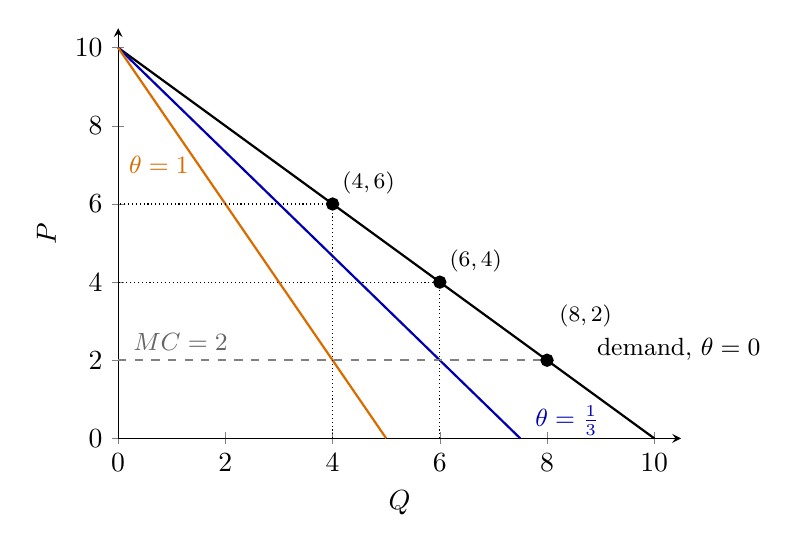
\begin{tikzpicture}
\begin{axis}[
  width=0.72\linewidth, height=0.56\linewidth,
  xmin=0, xmax=10.5, ymin=0, ymax=10.5,
  xlabel={$Q$}, ylabel={$P$},
  xtick={0,2,4,6,8,10}, ytick={0,2,4,6,8,10},
  axis lines=left, every axis plot/.append style={thick}, clip=false]
  \addplot[domain=0:10, samples=2, black] {10 - x};
  \node[anchor=south west, font=\small] at (axis cs:8.75,1.75) {demand, $\theta = 0$};
  \addplot[domain=0:7.5, samples=2, blue!70!black] {10 - (4/3)*x};
  \node[anchor=west, blue!70!black, font=\small] at (axis cs:7.6,0.45) {$\theta = \frac{1}{3}$};
  \addplot[domain=0:5, samples=2, orange!85!black] {10 - 2*x};
  \node[anchor=east, orange!85!black, font=\small] at (axis cs:1.5,7.0) {$\theta = 1$};
  \addplot[domain=0:8, samples=2, gray, dashed] {2};
  \node[anchor=south west, gray!80!black, font=\small] at (axis cs:0.1,2) {$MC = 2$};
  \addplot[only marks, mark=*, mark size=2pt] coordinates {(8,2) (6,4) (4,6)};
  \draw[densely dotted] (axis cs:6,0) -- (axis cs:6,4) -- (axis cs:0,4);
  \draw[densely dotted] (axis cs:4,0) -- (axis cs:4,6) -- (axis cs:0,6);
  \node[anchor=south west, font=\footnotesize] at (axis cs:8.05,2.6) {$(8, 2)$};
  \node[anchor=south west, font=\footnotesize] at (axis cs:6,4) {$(6, 4)$};
  \node[anchor=south west, font=\footnotesize] at (axis cs:4,6) {$(4, 6)$};
\end{axis}
\end{tikzpicture}
\caption{Perceived marginal revenue $10 - (1 + \theta)Q$ for demand $P = 10 - Q$ and $MC = 2$. Price taking
($\theta = 0$, perceived marginal revenue equal to demand) gives $Q = 8$ and $P = 2$. Conduct $\theta = \frac{1}{3}$,
as in a Stackelberg duopoly or a symmetric Cournot triopoly, gives $Q = 6$ and $P = 4$. Monopoly ($\theta = 1$)
gives $Q = 4$ and $P = 6$. In general $Q = \frac{8}{1 + \theta}$.}
\label{fig:02-perceived-mr}
\end{figure}

\subsection{Interpreting the conduct parameter}\label{sec:02-interpret}

\citet[Sec.~2.2]{Bresnahan1989} distinguishes three ways in which empirical work has used $\theta$.

The first takes $\theta$ from a single theory \citep[Sec.~2.2.1]{Bresnahan1989}. \citet{Rosse1970} estimates the
supply relation of monopoly newspapers ($\theta = 1$). His marginal revenue includes the effect of circulation on
advertising prices, and he infers marginal cost from $MR = MC$. Cournot models set $\tilde\theta_i = 1$
\citep[eq.~(6)]{Bresnahan1989}. Stackelberg and dominant-firm models give the leader the values derived above.
Dynamic theories of collusion imply a $\theta$ that switches between regimes, as in \citet{Porter1983}. In all these
cases the theory fixes the value or the pattern of $\theta$ before the data are consulted.

The second approach estimates the supply relations of a few distinct theories and tests them against each other
\citep[Sec.~2.2.2]{Bresnahan1989}. \citet{Bresnahan1987} compares joint-profit pricing with Bertrand pricing in the
automobile industry of the mid-1950s. He finds collusive behavior in some years and Bertrand behavior in 1955
(\cref{ch:discrete}). Bresnahan stresses that this approach differs from estimating a continuous $\theta$ only
econometrically. A continuous $\theta$ leads to nested tests, while a few discrete theories lead to non-nested tests.

The third approach treats $\theta$ as a continuous parameter described as a ``conjectural variation''
\citep[Sec.~2.2.3]{Bresnahan1989}. \citet{Iwata1974} used it to locate the Japanese plate-glass industry between
competition and monopoly. Since $\tilde\theta_i - 1 = r_i$ is an identity, saying what the conjectural variation is
and saying which oligopoly theory fits the data are the same statement \citep[p.~1027]{Bresnahan1989}.

\casehead{The critique of conjectural variations} Taken literally, a conjecture describes how a firm expects rivals
to react to a change in its output. In a simultaneous-move game nobody can react, so any nonzero conjecture is
inconsistent with the game being played. \emph{Consistent conjectures}, which require each conjecture to equal the
actual slope of rivals' responses, were one attempted repair \citep{Bresnahan1981a}. They keep the static framework
and have not become standard. \citet[pp.~1028--1029]{Bresnahan1989} offers a different reading. Collusive conduct
$\tilde\theta_i = N$ would literally mean that each firm expects rivals to match any output change one for one. In
repeated-game models firms produce the collusive output for another reason. They expect a deviation to trigger a
general breakdown of restraint. An estimated $\theta$ therefore describes what firms do. It does not reveal what they
believe would happen after a deviation. If $\theta$ is stable and breakdowns are rare, it measures the average collusiveness of
conduct. It tells us nothing about firms' expectations beyond the fact that they deter deviations
\citep[n.~19]{Bresnahan1989}.

A more basic problem is that an unrestricted $\theta$ explains everything.

\begin{proposition}[Exact fit]\label{prop:02-theta-fit}
Let $(P_{it}, Q_{it})$, with $Q_{it} > 0$, be data on prices and quantities. Take any demand system with slope
$\frac{\partial Q_{it}}{\partial P_{it}} < 0$ at each observation and any marginal cost function, with implied
values $mc_{it}$. Setting
\begin{equation*}
\theta_{it} = \frac{\left(P_{it} - mc_{it}\right)\left|\frac{\partial Q_{it}}{\partial P_{it}}\right|}{Q_{it}}
\end{equation*}
makes the supply relation
\[
P_{it} = mc_{it} + \theta_{it}\frac{Q_{it}}{\left|\frac{\partial Q_{it}}{\partial P_{it}}\right|}
\]
hold exactly at every observation, with no error term. The implied $\theta_{it}$ is nonnegative whenever
$mc_{it} \le P_{it}$.
\end{proposition}

\begin{proof}
Substituting the stated $\theta_{it}$ into the right side of the supply relation gives
\[
mc_{it} + \frac{(P_{it} - mc_{it})\left|\frac{\partial Q_{it}}{\partial P_{it}}\right|}{Q_{it}}
\cdot\frac{Q_{it}}{\left|\frac{\partial Q_{it}}{\partial P_{it}}\right|} = mc_{it} + (P_{it} - mc_{it}) = P_{it} . \qedhere
\]
\end{proof}

The supply relation has empirical content only through restrictions on $\theta$. The usual ones are that $\theta$ is
constant across observations or groups, or that $\theta \in [0, 1]$. Others fix $\theta$ at the value implied by a
specific game, or require deviations of $\theta$ to be uncorrelated with the instruments. Each restriction is an assumption, and
each objection to a conduct study is an objection to one of them. Imposing a functional form on marginal cost does not
help by itself, since the proposition holds for every cost function.

\casehead{The conduct parameter as a specification test} \citet[p.~1031]{Bresnahan1989} credits
\citet{Appelbaum1979} with a useful observation. Setting $\theta = 0$ in \eqref{eq:02-supply-relation} imposes price
taking. Every approach to conduct is therefore a test of price taking against alternatives with market power. A
cautious use of $\theta$ follows. We estimate it freely and test the hypotheses $\theta = 0$,
$\theta = \frac{1}{N}$ and $\theta = 1$, without reading $\hat\theta$ as a deep behavioral parameter. Even this use
requires care. If true conduct varies with demand, as in repeated-game models, an instrumental-variables estimate of a
constant $\theta$ measures how the markup responds to demand shifts. It need not equal average conduct, a point due to
\citet{Corts1999} and developed in \cref{ch:conduct}.

\casehead{Observed marginal cost} When marginal cost can be measured directly, \eqref{eq:02-theta-lerner} delivers
conduct observation by observation, $\theta_t = \varepsilon_t\frac{P_t - MC_t}{P_t}$, once demand is known. A known
cost structure serves a similar purpose. Fixed-proportions technology, for example, pins marginal cost down up to one
or two parameters, which can be estimated jointly with $\theta$. These are the strategies of \citet{Wolfram1999} for
electricity and \citet{GenesoveMullin1998} for sugar refining. Both compare the direct measure with the estimate a
researcher would obtain without cost data (\cref{ch:conduct}).

\subsection{Forward contracts}\label{sec:02-forward}

Contracts signed before the spot market opens change the spot-market incentive to raise price. The case matters for
electricity markets, where most output is often sold forward.

\begin{example}[Cournot with forward sales]\label{ex:02-forward}
Suppose firm $i$ has sold $x_i$ units forward at price $p^f$, before the spot market opens. Its spot-market profit is
\begin{equation*}
P(Q)\left(q_i - x_i\right) + p^f x_i - C_i(q_i) .
\end{equation*}
The forward revenue $p^f x_i$ is fixed, and only the uncontracted output $q_i - x_i$ earns the spot price. The Cournot
first-order condition is
\begin{equation*}
P(Q) + \left(q_i - x_i\right) P'(Q) = C_i'(q_i) .
\end{equation*}
Using $-P' = \frac{P}{\varepsilon Q}$ and dividing by $P$,
\begin{equation}\label{eq:02-forward-lerner}
\frac{P - C_i'(q_i)}{P} = \frac{q_i - x_i}{Q}\cdot\frac{1}{\varepsilon}
= \frac{s_i}{\varepsilon}\left(1 - \frac{x_i}{q_i}\right) .
\end{equation}
In conduct terms, $\tilde\theta_i = 1 - \frac{x_i}{q_i}$. A firm with 80 percent of its output under contract has
one fifth of the Cournot incentive to raise the spot price.
\end{example}

\citet{AllazVila1993} show that firms also have a strategic reason to sell forward. A forward sale commits a firm to
a higher spot output. Since quantities are strategic substitutes, rivals respond by producing less. Every firm has
this incentive, and together they end up in a prisoners' dilemma that lowers prices. In the linear duopoly with
$P = a - bQ$ and cost $c$, suppose arbitrage makes the forward price equal the spot price. The spot stage gives
$q_i = \frac{a - c + 2b x_i - b x_j}{3b}$ and $P - c = \frac{a - c - b(x_1 + x_2)}{3}$. Each firm then chooses $x_i$
to maximize $(P - c)\, q_i$. The first-order condition is $a - c - 4b x_i - b x_j = 0$, so the symmetric solution is
$x_i = \frac{a - c}{5b}$. Spot outputs are $q_i = \frac{2(a - c)}{5b}$, half of output is sold forward, and
$P - c = \frac{a - c}{5}$. Without a forward market, Cournot gives $P - c = \frac{a - c}{3}$. As a check,
\eqref{eq:02-forward-lerner} with $s_i = \frac{1}{2}$ and $\frac{x_i}{q_i} = \frac{1}{2}$ gives
$P - c = \frac{1}{4}\, b Q = \frac{a - c}{5}$. \Cref{ch:conduct} returns to contract cover in the British electricity
market.

\begin{remark}[Very inelastic demand]\label{rem:02-inelastic}
By \cref{prop:02-cowling-waterson}, Cournot firm $i$ has $L_i = \frac{s_i}{\varepsilon}$. With constant-elasticity
demand, an interior equilibrium requires $L_i < 1$, that is, $s_i < \varepsilon$. When market demand is very inelastic, as in electricity, the static
Cournot model predicts no interior equilibrium. Firms would withhold output until a capacity constraint binds. In such
markets prices are held down by something outside the static model. Capacity limits, regulatory threats, forward
contracts and the threat of entry are the usual candidates.
\end{remark}

\subsection{Pricing rules for the Bulow-Pfleiderer family}\label{sec:02-bp-rules}

The supply relation yields closed-form pricing rules for the demand family $Q(p) = B(\bar p - p)^{g}$ of
\cref{ex:02-bp}. With constant marginal cost $c$, the derivation has three steps.

First, compute $q\,P'(q)$. Since $P'(q) = \frac{1}{Q'(p)}$ and $Q'(p) = -gB(\bar p - p)^{g - 1}$,
\begin{equation*}
q\,P'(q) = \frac{Q(p)}{Q'(p)} = \frac{B(\bar p - p)^{g}}{-gB(\bar p - p)^{g - 1}} = -\frac{\bar p - p}{g} .
\end{equation*}
Second, substitute into $p + \theta q P'(q) = c$:
\begin{equation*}
p - \frac{\theta(\bar p - p)}{g} = c
\quad\Longrightarrow\quad
g p + \theta p = g c + \theta \bar p .
\end{equation*}
Third, solve for $p$:
\begin{equation}\label{eq:02-gm-rule}
P(c;\theta) = \frac{\theta\bar p + g c}{g + \theta} .
\end{equation}
Monopoly ($\theta = 1$) gives $P(c;1) = \frac{\bar p + gc}{1 + g}$, the rule of \cref{ex:02-bp}. Price taking
gives $P(c;0) = c$. The rule nests the other families as limits.
\begin{itemize}
\item Linear demand ($g = 1$) gives $P = \frac{\theta\bar p + c}{1 + \theta}$, and quadratic demand ($g = 2$)
  gives $P = \frac{\theta\bar p + 2c}{2 + \theta}$.
\item Constant elasticity ($\bar p = 0$ and $g = -\varepsilon < 0$) gives $P = \frac{gc}{g + \theta}
  = \frac{\varepsilon}{\varepsilon - \theta}\, c$, which requires $\varepsilon > \theta$.
\item In the exponential limit, $g$ and $\bar p$ grow without bound with $\frac{g}{\bar p} = \lambda_s$ fixed. Demand tends to
  $Q \propto e^{-\lambda_s p}$, with constant semi-elasticity $\lambda_s$. Since $\frac{\bar p - p}{g} =
  \frac{1}{\lambda_s} - \frac{p}{g} \to \frac{1}{\lambda_s}$, the rule becomes $P = c + \frac{\theta}{\lambda_s}$, a
  constant dollar markup.
\end{itemize}
The cost slope of \eqref{eq:02-gm-rule} is $\frac{\partial P}{\partial c} = \frac{g}{g + \theta}$, which depends on
conduct and curvature together (\cref{sec:02-passthrough}). The intercept $\frac{\theta\bar p}{g + \theta}$ moves
with the demand parameter $\bar p$. A season in which demand rotates, changing $\bar p$ or $g$, therefore shifts price
by an amount that rises with $\theta$ and vanishes at $\theta = 0$. \citet{GenesoveMullin1998} estimate exactly these rules for sugar refining and
use such a seasonal rotation to identify conduct (\cref{ch:conduct}).
